\documentclass[11pt, letterpaper]{article}

% Fonts and Encoding
\usepackage[utf8]{inputenc}
\usepackage[T1]{fontenc}
\usepackage{lmodern} % High-quality Latin Modern vector font

% Math and Symbols
\usepackage{amsmath, amssymb, amsthm, amsfonts, mathrsfs, mathtools}

% Layout and Geometry
\usepackage{geometry}
\geometry{letterpaper, margin=1in}
\setlength{\parindent}{0pt}
\setlength{\parskip}{0.6em}

% Formatting and Graphics
\usepackage{graphicx, xcolor, enumitem, booktabs, array, tabularx}

% TikZ for Illustrations
\usepackage{tikz}
\usetikzlibrary{arrows.meta, positioning, shapes.geometric, calc, backgrounds, matrix}

% Clickable Links and TOC
\usepackage{hyperref}
\hypersetup{
    colorlinks=true,
    linkcolor=blue,
    filecolor=magenta,      
    urlcolor=cyan,
    pdftitle={Advanced Mathematics Topic},
}

% Theorem Environments
\newtheorem{theorem}{Theorem}[section]
\newtheorem{lemma}[theorem]{Lemma}
\newtheorem{proposition}[theorem]{Proposition}
\newtheorem{corollary}[theorem]{Corollary}
\theoremstyle{definition}
\newtheorem{definition}{Definition}[section]
\newtheorem{axiom}{Axiom}[section]
\newtheorem{example}{Example}[section]
\theoremstyle{remark}
\newtheorem{remark}{Remark}[section]

% Custom Commands (Enforced standard notation)
\newcommand{\R}{\mathbb{R}}
\newcommand{\N}{\mathbb{N}}
\newcommand{\Z}{\mathbb{Z}}
\newcommand{\Q}{\mathbb{Q}}
\newcommand{\E}{\mathbb{E}}
\newcommand{\Prob}{\mathbb{P}}
\newcommand{\F}{\mathcal{F}}

\title{\textbf{Mastering Constrained Optimization of Quadratic Forms}\\
\large Comprehensive Theory, Complete Analytical Solutions, and Applied Spectral Modeling (Section 7.3)}
\author{Tashfeen Omran}
\date{\today}

\begin{document}

\maketitle
\tableofcontents
\newpage

% ============================================================================
% PART 1: COMPREHENSIVE INTRODUCTION, CONTEXT, AND PREREQUISITES
% ============================================================================
\section{Comprehensive Introduction, Context, and Prerequisites}

\subsection{Core Concepts and Problem Formulation}

Across engineering, economics, physics, and data science, one frequently needs to determine the extreme values (maximum or minimum) of a quadratic form $Q(\mathbf{x}) = \mathbf{x}^T A \mathbf{x}$ when the input vector $\mathbf{x} \in \mathbb{R}^n$ is restricted to lie in a prescribed constraint set. Without any restriction on $\mathbf{x}$, scaling a vector by a real scalar $c \in \mathbb{R}$ scales the quadratic form quadratically:
\[
Q(c\mathbf{x}) = (c\mathbf{x})^T A (c\mathbf{x}) = c^2 (\mathbf{x}^T A \mathbf{x}) = c^2 Q(\mathbf{x}).
\]
Consequently, whenever $Q(\mathbf{x})$ takes at least one positive value, $Q(c\mathbf{x}) \to +\infty$ as $|c| \to \infty$, so no finite global maximum exists on $\mathbb{R}^n$. Instead, the mathematically natural and physically meaningful problem is to optimize $Q(\mathbf{x})$ over all \emph{directions} in $\mathbb{R}^n$, which corresponds to restricting $\mathbf{x}$ to the set of \textbf{unit vectors} (the unit sphere $S^{n-1} \subset \mathbb{R}^n$).

\begin{definition}[Unit-Vector Constraint Formulations]
For a vector $\mathbf{x} = (x_1, x_2, \dots, x_n)^T \in \mathbb{R}^n$, the requirement that $\mathbf{x}$ be a unit vector can be stated in four algebraically equivalent ways:
\[
\|\mathbf{x}\| = 1, \qquad \|\mathbf{x}\|^2 = 1, \qquad \mathbf{x}^T \mathbf{x} = 1, \qquad x_1^2 + x_2^2 + \cdots + x_n^2 = 1.
\]
\end{definition}

Throughout constrained optimization of quadratic forms, $A$ denotes an $n \times n$ real \textbf{symmetric matrix} ($A^T = A$). By the Extreme Value Theorem of multivariable analysis (and algebraically via Exercise 13), because $Q(\mathbf{x}) = \mathbf{x}^T A \mathbf{x}$ is continuous and the unit sphere $\{\mathbf{x} \in \mathbb{R}^n : \|\mathbf{x}\| = 1\}$ is closed, bounded, and path-connected (for $n \ge 2$), the set of all values attained by $\mathbf{x}^T A \mathbf{x}$ for $\|\mathbf{x}\| = 1$ forms a closed, bounded interval $[m, M] \subset \mathbb{R}$, where:
\[
m = \min \{\mathbf{x}^T A \mathbf{x} : \|\mathbf{x}\| = 1\}, \qquad M = \max \{\mathbf{x}^T A \mathbf{x} : \|\mathbf{x}\| = 1\}.
\]

\begin{remark}[Natural Real Ordering Versus Magnitude]
The terms \emph{minimum}, \emph{maximum}, \emph{least}, and \emph{greatest} always refer to the standard ordering of real numbers on the number line ($-\infty < \cdots < -5 < -1 < 0 < 1 < 5 < \cdots < +\infty$), \textbf{never} to absolute values or magnitudes. For instance, if the eigenvalues of $A$ are $1$, $-2$, and $-6$, the greatest eigenvalue is $M = 1$ and the least eigenvalue is $m = -6$. If the eigenvalues of $A$ are $-4$, $-10$, $-12$, and $-16$, the greatest eigenvalue is $M = -4$.
\end{remark}

Beyond finding the overall maximum $M$ and minimum $m$ on the unit sphere, Section 7.3 introduces \textbf{sequential orthogonality constraints}. Once a unit vector $\mathbf{u}_1$ maximizing $Q(\mathbf{x})$ on the unit sphere has been found, we often seek the next most dominant independent direction by maximizing $Q(\mathbf{x})$ over all unit vectors $\mathbf{x}$ orthogonal to $\mathbf{u}_1$:
\[
\mathbf{x}^T \mathbf{x} = 1 \quad \text{and} \quad \mathbf{x}^T \mathbf{u}_1 = 0.
\]
More generally, given orthonormal eigenvectors $\mathbf{u}_1, \mathbf{u}_2, \dots, \mathbf{u}_{k-1}$ corresponding to the top $k-1$ eigenvalues $\lambda_1 \ge \lambda_2 \ge \cdots \ge \lambda_{k-1}$, imposing the simultaneous constraints $\mathbf{x}^T \mathbf{x} = 1$ and $\mathbf{x}^T \mathbf{u}_1 = \cdots = \mathbf{x}^T \mathbf{u}_{k-1} = 0$ isolates the $k$-th eigenvalue $\lambda_k$.

\subsection{Geometric Intuition and Mathematical Derivation}

To understand \emph{why} the constrained extrema of $Q(\mathbf{x}) = \mathbf{x}^T A \mathbf{x}$ on $\|\mathbf{x}\| = 1$ coincide exactly with the eigenvalues of $A$, we proceed in two transparent steps: first analyzing a diagonal quadratic form (no cross-product terms), and then reducing every symmetric quadratic form to the diagonal case via an orthogonal change of coordinates.

\paragraph{Step 1: The Diagonal Case (Uncoupled Coordinates).}
Suppose $D = \operatorname{diag}(\lambda_1, \lambda_2, \dots, \lambda_n)$ with diagonal entries ordered so that $\lambda_1 \ge \lambda_2 \ge \cdots \ge \lambda_n$. For any unit vector $\mathbf{y} = (y_1, y_2, \dots, y_n)^T \in \mathbb{R}^n$ satisfying $y_1^2 + y_2^2 + \cdots + y_n^2 = 1$, every square $y_i^2 \ge 0$ is nonnegative. Multiplying the inequalities $\lambda_n \le \lambda_i \le \lambda_1$ by $y_i^2 \ge 0$ gives $\lambda_n y_i^2 \le \lambda_i y_i^2 \le \lambda_1 y_i^2$ for each $i = 1, \dots, n$. Summing over $i$ yields:
\begin{align*}
\mathbf{y}^T D \mathbf{y} &= \lambda_1 y_1^2 + \lambda_2 y_2^2 + \cdots + \lambda_n y_n^2 \\
&\le \lambda_1 y_1^2 + \lambda_1 y_2^2 + \cdots + \lambda_1 y_n^2 = \lambda_1 (y_1^2 + y_2^2 + \cdots + y_n^2) = \lambda_1 (1) = \lambda_1.
\end{align*}
Similarly, bounding below by $\lambda_n$ gives:
\[
\mathbf{y}^T D \mathbf{y} \ge \lambda_n y_1^2 + \lambda_n y_2^2 + \cdots + \lambda_n y_n^2 = \lambda_n (y_1^2 + y_2^2 + \cdots + y_n^2) = \lambda_n.
\]
Hence $\lambda_n \le \mathbf{y}^T D \mathbf{y} \le \lambda_1$ for every unit vector $\mathbf{y}$. Crucially, both bounds are actually \emph{attained}:
\begin{itemize}[leftmargin=2em]
    \item Choosing $\mathbf{y} = \mathbf{e}_1 = (1, 0, \dots, 0)^T$ yields $\mathbf{e}_1^T D \mathbf{e}_1 = \lambda_1(1)^2 + 0 = \lambda_1$.
    \item Choosing $\mathbf{y} = \mathbf{e}_n = (0, \dots, 0, 1)^T$ yields $\mathbf{e}_n^T D \mathbf{e}_n = \lambda_n(1)^2 = \lambda_n$.
\end{itemize}
Notice that $\mathbf{y}^T D \mathbf{y}$ is a \emph{weighted average} (convex combination) of the eigenvalues $\lambda_1, \dots, \lambda_n$ with nonnegative weights $w_i = y_i^2$ summing to $1$. To maximize a weighted average of numbers, one places $100\%$ of the weight on the largest number ($y_1^2 = 1$, all other $y_i = 0$).

\paragraph{Step 2: General Symmetric Matrices via Orthogonal Diagonalization.}
Now let $A$ be any real symmetric $n \times n$ matrix. By the Spectral Theorem for Symmetric Matrices (Section 7.1), $A$ is orthogonally diagonalizable: there exists an orthogonal matrix $P = \begin{bmatrix} \mathbf{u}_1 & \mathbf{u}_2 & \cdots & \mathbf{u}_n \end{bmatrix}$ (satisfying $P^T P = I$, so $P^{-1} = P^T$) and a diagonal matrix $D = \operatorname{diag}(\lambda_1, \lambda_2, \dots, \lambda_n)$ with $\lambda_1 \ge \lambda_2 \ge \cdots \ge \lambda_n$ such that $A = P D P^T$. Make the orthogonal change of variable $\mathbf{x} = P\mathbf{y}$:
\begin{enumerate}[leftmargin=2em]
    \item \textbf{Objective Transformation:} $\mathbf{x}^T A \mathbf{x} = (P\mathbf{y})^T A (P\mathbf{y}) = \mathbf{y}^T (P^T A P) \mathbf{y} = \mathbf{y}^T D \mathbf{y}$.
    \item \textbf{Constraint Preservation (Isometry):} Because $P^T P = I$, the transformation $\mathbf{x} = P\mathbf{y}$ preserves lengths and inner products:
    \[
    \|\mathbf{x}\|^2 = \|P\mathbf{y}\|^2 = (P\mathbf{y})^T (P\mathbf{y}) = \mathbf{y}^T P^T P \mathbf{y} = \mathbf{y}^T I \mathbf{y} = \mathbf{y}^T \mathbf{y} = \|\mathbf{y}\|^2.
    \]
    Therefore, $\|\mathbf{x}\| = 1$ if and only if $\|\mathbf{y}\| = 1$. As $\mathbf{y}$ ranges over the unit sphere, $\mathbf{x} = P\mathbf{y}$ ranges bijectively over the exact same unit sphere!
\end{enumerate}
Combining Steps 1 and 2 immediately proves that $\max_{\|\mathbf{x}\|=1} \mathbf{x}^T A \mathbf{x} = \max_{\|\mathbf{y}\|=1} \mathbf{y}^T D \mathbf{y} = \lambda_1$, attained when $\mathbf{y} = \mathbf{e}_1$, which translates back into $\mathbf{x}$-coordinates as:
\[
\mathbf{x} = P\mathbf{e}_1 = \begin{bmatrix} \mathbf{u}_1 & \mathbf{u}_2 & \cdots & \mathbf{u}_n \end{bmatrix} \begin{bmatrix} 1 \\ 0 \\ \vdots \\ 0 \end{bmatrix} = \mathbf{u}_1.
\]
Likewise, $\min_{\|\mathbf{x}\|=1} \mathbf{x}^T A \mathbf{x} = \lambda_n$, attained at $\mathbf{x} = P\mathbf{e}_n = \mathbf{u}_n$.

Furthermore, if we impose the additional orthogonality constraints $\mathbf{x}^T \mathbf{u}_1 = 0, \dots, \mathbf{x}^T \mathbf{u}_{k-1} = 0$, notice that since $\mathbf{u}_j = P\mathbf{e}_j$ and $P^T P = I$:
\[
\mathbf{x}^T \mathbf{u}_j = (P\mathbf{y})^T (P\mathbf{e}_j) = \mathbf{y}^T P^T P \mathbf{e}_j = \mathbf{y}^T \mathbf{e}_j = y_j = 0 \qquad (j = 1, \dots, k-1).
\]
With $y_1 = \cdots = y_{k-1} = 0$, the quadratic form collapses to $\mathbf{y}^T D \mathbf{y} = \lambda_k y_k^2 + \cdots + \lambda_n y_n^2$ subject to $y_k^2 + \cdots + y_n^2 = 1$. Its maximum is manifestly $\lambda_k$, attained at $\mathbf{y} = \mathbf{e}_k$, i.e., $\mathbf{x} = P\mathbf{e}_k = \mathbf{u}_k$.

\begin{center}
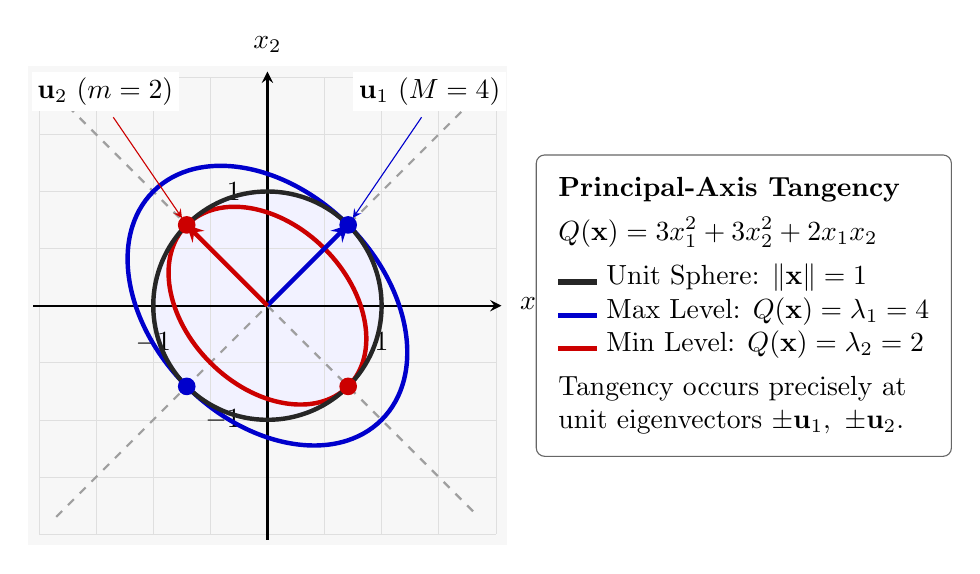
\begin{tikzpicture}[scale=1.45]
    % 1) Backgrounds
    \fill[gray!6] (-2.1,-2.1) rectangle (2.1,2.1);
    \fill[blue!5] (0,0) circle (1);

    % 2) Grid lines and Axes
    \draw[step=0.5, gray!25, very thin] (-2.0,-2.0) grid (2.0,2.0);
    \draw[->, >=stealth, thick, black] (-2.05,0) -- (2.05,0) node[right=3pt, text=black] {$x_1$};
    \draw[->, >=stealth, thick, black] (0,-2.05) -- (0,2.05) node[above=3pt, text=black] {$x_2$};

    % Principal axes dashed lines
    \draw[dashed, gray!75, thick] (-1.85,-1.85) -- (1.85,1.85);
    \draw[dashed, gray!75, thick] (-1.85,1.85) -- (1.85,-1.85);

    % Explicit microscopic tick marks
    \draw[thick, black] (1,0) -- (1,-0.07) node[below=3pt, text=black] {$1$};
    \draw[thick, black] (-1,0) -- (-1,-0.07) node[below=3pt, text=black] {$-1$};
    \draw[thick, black] (0,1) -- (-0.07,1) node[left=3pt, text=black] {$1$};
    \draw[thick, black] (0,-1) -- (-0.07,-1) node[left=3pt, text=black] {$-1$};

    % 3) Primary Plots: Unit Circle and Tangent Level Curves of Q(x) = 3x_1^2 + 3x_2^2 + 2x_1x_2
    % In rotated frame (45 deg): 4y_1^2 + 2y_2^2 = c
    % c = 4 (Max): y_1^2/1 + y_2^2/2 = 1 -> semi-axes 1 and sqrt(2)=1.4142
    \draw[ultra thick, blue!80!black, rotate=45] (0,0) ellipse (1 and 1.4142);
    % c = 2 (Min): y_1^2/(0.5) + y_2^2/1 = 1 -> semi-axes 0.7071 and 1
    \draw[ultra thick, red!80!black, rotate=45] (0,0) ellipse (0.7071 and 1);
    % Unit Circle: x_1^2 + x_2^2 = 1
    \draw[ultra thick, black!85] (0,0) circle (1);

    % Principal Eigenvector Arrows
    \draw[->, >=stealth, ultra thick, blue!80!black] (0,0) -- (0.7071,0.7071);
    \draw[->, >=stealth, ultra thick, red!80!black] (0,0) -- (-0.7071,0.7071);

    % Tangency Dots
    \fill[blue!80!black] (0.7071,0.7071) circle (2.2pt);
    \fill[blue!80!black] (-0.7071,-0.7071) circle (2.2pt);
    \fill[red!80!black] (-0.7071,0.7071) circle (2.2pt);
    \fill[red!80!black] (0.7071,-0.7071) circle (2.2pt);

    % Off-Axis Callout Arrows
    \draw[->, >=stealth, shorten >=3pt, thin, blue!80!black] (1.35,1.65) -- (0.7071,0.7071);
    \draw[->, >=stealth, shorten >=3pt, thin, red!80!black] (-1.35,1.65) -- (-0.7071,0.7071);

    % 4) Labels and Single-Node Legend
    \node[above=2pt, text=black, fill=white, inner sep=2pt] at (1.42,1.65) {$\mathbf{u}_1 \ (M=4)$};
    \node[above=2pt, text=black, fill=white, inner sep=2pt] at (-1.42,1.65) {$\mathbf{u}_2 \ (m=2)$};

    \node[draw=black!60, fill=white, rounded corners=3pt, align=left, inner sep=8pt, text=black, anchor=west] at (2.35, 0) {
        \textbf{Principal-Axis Tangency}\\[4pt]
        $\displaystyle Q(\mathbf{x}) = 3x_1^2 + 3x_2^2 + 2x_1 x_2$\\[4pt]
        \textcolor{black!85}{\rule{14pt}{2pt}} Unit Sphere: $\displaystyle \|\mathbf{x}\| = 1$\\
        \textcolor{blue!80!black}{\rule{14pt}{2pt}} Max Level: $\displaystyle Q(\mathbf{x}) = \lambda_1 = 4$\\
        \textcolor{red!80!black}{\rule{14pt}{2pt}} Min Level: $\displaystyle Q(\mathbf{x}) = \lambda_2 = 2$\\[4pt]
        Tangency occurs precisely at\\
        unit eigenvectors $\displaystyle \pm\mathbf{u}_1,\ \pm\mathbf{u}_2$.
    };
\end{tikzpicture}
\end{center}

\subsection{Historical Context and Scientific Motivation}

The constrained optimization of quadratic forms emerged in the eighteenth and nineteenth centuries from two foundational problems in mathematical physics: \emph{rigid-body mechanics} and \emph{celestial perturbation theory}. Leonhard Euler (1760) discovered that the rotational kinetic energy of a three-dimensional rigid body spinning with angular velocity $\boldsymbol{\omega}$ of unit magnitude is governed by a quadratic form $\boldsymbol{\omega}^T I \boldsymbol{\omega}$, where $I$ is the symmetric inertia tensor; finding the stable axes of maximal and minimal rotational inertia required locating the constrained extrema of $\boldsymbol{\omega}^T I \boldsymbol{\omega}$ on the unit sphere $\|\boldsymbol{\omega}\| = 1$. Nearly seventy years later, Augustin-Louis Cauchy (1829), motivated by Pierre-Simon Laplace and Joseph-Louis Lagrange's investigations into the long-term secular stability of planetary orbits, proved that every real symmetric matrix possesses exclusively real eigenvalues and mutually orthogonal principal axes by analyzing the points on a quadric surface closest to and farthest from the origin.

In the late nineteenth and early twentieth centuries, this geometric extremal principle became the cornerstone of modern mathematical physics and functional analysis. In *The Theory of Sound* (1877), John William Strutt (Lord Rayleigh) introduced the \textbf{Rayleigh quotient} $R(\mathbf{x}) = (\mathbf{x}^T A \mathbf{x}) / (\mathbf{x}^T \mathbf{x})$ as a powerful variational tool to approximate the fundamental resonant frequencies of vibrating membranes and elastic structures without solving high-degree characteristic polynomials directly. Ernst Fischer (1905) and Richard Courant (1920) subsequently generalized Rayleigh's principle to characterize all higher eigenvalues via sequential orthogonality and subspace min-max constraints—a breakthrough that provided the rigorous mathematical foundation for quantized energy levels in Erwin Schr\"odinger's wave mechanics (1926) and Karl Pearson and Harold Hotelling's Principal Component Analysis (1901, 1933) in multivariate statistics.

\subsection{Summary of Essential Theorems and Formulas}

We formally state the three central theorems of Section 7.3 together with a unified reference table of key identities.

\begin{theorem}[Theorem 6: Constrained Extrema on the Unit Sphere]\label{thm:thm6}
Let $A$ be a real symmetric $n \times n$ matrix, and define
\[
m = \min \{\mathbf{x}^T A \mathbf{x} : \|\mathbf{x}\| = 1\}, \qquad M = \max \{\mathbf{x}^T A \mathbf{x} : \|\mathbf{x}\| = 1\}.
\]
Then $M$ is the greatest eigenvalue $\lambda_1$ of $A$, and $m$ is the least eigenvalue $\lambda_n$ of $A$. Moreover, the value of $\mathbf{x}^T A \mathbf{x}$ is $M$ when $\mathbf{x}$ is a unit eigenvector $\mathbf{u}_1$ corresponding to $M$, and the value of $\mathbf{x}^T A \mathbf{x}$ is $m$ when $\mathbf{x}$ is a unit eigenvector $\mathbf{u}_n$ corresponding to $m$.
\end{theorem}

\begin{theorem}[Theorem 7: Second Greatest Eigenvalue Under Orthogonality]\label{thm:thm7}
Let $A$, $\lambda_1$, and $\mathbf{u}_1$ be as in Theorem~\ref{thm:thm6} (with eigenvalues ordered $\lambda_1 \ge \lambda_2 \ge \cdots \ge \lambda_n$). Then the maximum value of $\mathbf{x}^T A \mathbf{x}$ subject to the constraints
\[
\mathbf{x}^T \mathbf{x} = 1, \qquad \mathbf{x}^T \mathbf{u}_1 = 0
\]
is the second greatest eigenvalue, $\lambda_2$, and this maximum is attained when $\mathbf{x}$ is a unit eigenvector $\mathbf{u}_2$ corresponding to $\lambda_2$.
\end{theorem}

\begin{theorem}[Theorem 8: Variational Characterization of All Eigenvalues]\label{thm:thm8}
Let $A$ be a symmetric $n \times n$ matrix with an orthogonal diagonalization $A = P D P^{-1}$, where the entries on the diagonal of $D$ are arranged so that $\lambda_1 \ge \lambda_2 \ge \cdots \ge \lambda_n$ and where the columns of $P$ are corresponding unit eigenvectors $\mathbf{u}_1, \dots, \mathbf{u}_n$. Then for $k = 2, \dots, n$, the maximum value of $\mathbf{x}^T A \mathbf{x}$ subject to the constraints
\[
\mathbf{x}^T \mathbf{x} = 1, \qquad \mathbf{x}^T \mathbf{u}_1 = 0, \quad \dots, \quad \mathbf{x}^T \mathbf{u}_{k-1} = 0
\]
is the eigenvalue $\lambda_k$, and this maximum is attained at $\mathbf{x} = \mathbf{u}_k$.
\end{theorem}

\renewcommand{\arraystretch}{1.5}
\begin{tabularx}{\textwidth}{l >{$\displaystyle}l<{$} X}
\toprule
\textbf{Concept} & \multicolumn{1}{l}{\textbf{Canonical Formula}} & \textbf{Explanation and Role} \\
\midrule
Symmetric Matrix of $Q$ & Q(\mathbf{x}) = \sum_{i=1}^n a_{ii} x_i^2 + 2\sum_{i < j} a_{ij} x_i x_j^{\vphantom{A}} & Diagonal entries are squared coefficients; off-diagonal entries $a_{ij} = a_{ji}$ are \textbf{half} the $x_i x_j$ cross-product coefficients. \\
\addlinespace[4pt]
Orthogonal Substitution & \mathbf{x} = P\mathbf{y}, \quad P^T P = I & Decouples $Q(\mathbf{x}) = \mathbf{y}^T D \mathbf{y}$ while preserving norm $\|\mathbf{x}\| = \|\mathbf{y}\|$. \\
\addlinespace[4pt]
Unit-Sphere Bounds & \lambda_n \le \mathbf{x}^T A \mathbf{x} \le \lambda_1 \quad (\|\mathbf{x}\| = 1) & Image of the unit sphere under $Q$ is the closed interval $[m, M] = [\lambda_n, \lambda_1]$. \\
\addlinespace[4pt]
Rayleigh Quotient & R(\mathbf{x}) = \frac{\mathbf{x}^T A \mathbf{x}}{\mathbf{x}^T \mathbf{x}} \quad (\mathbf{x} \neq \mathbf{0}) & Scale-invariant form; normalizing $\mathbf{u} = \mathbf{x}/\|\mathbf{x}\|$ reduces $R(\mathbf{x})$ to $\mathbf{u}^T A \mathbf{u}$ on $\|\mathbf{u}\| = 1$. \\
\addlinespace[4pt]
Elliptical Scaling & \left(\frac{x_1}{c_1}\right)^2 + \left(\frac{x_2}{c_2}\right)^2 = 1 \implies \tilde{x}_i = \frac{x_i}{c_i} & Converts an ellipsoidal boundary into the unit sphere $\tilde{\mathbf{x}}^T \tilde{\mathbf{x}} = 1$. \\
\bottomrule
\end{tabularx}

\subsection{Essential Prerequisites}

To master Section 7.3 with complete fluency, the following foundational skills are indispensable:
\begin{enumerate}[leftmargin=2em]
    \item \textbf{Symmetric Matrix Construction (Section 7.2):} Accurately translating a scalar polynomial $Q(x_1, \dots, x_n)$ into $\mathbf{x}^T A \mathbf{x}$ with $A^T = A$ by placing $x_i^2$ coefficients on the main diagonal and splitting each $x_i x_j$ ($i \neq j$) coefficient equally between $a_{ij}$ and $a_{ji}$.
    \item \textbf{Characteristic Polynomials and Root Finding (Chapter 5):} Computing $\det(A - \lambda I) = 0$, factoring cubic or quartic polynomials (or applying the quadratic formula $\lambda = \frac{-b \pm \sqrt{b^2 - 4ac}}{2a}$ for $2 \times 2$ matrices), and exploiting matrix invariants such as $\operatorname{tr}(A) = \sum_{i=1}^n \lambda_i$ and $\det(A) = \prod_{i=1}^n \lambda_i$.
    \item \textbf{Null-Space Computation via Row Reduction:} Solving homogeneous linear systems $(A - \lambda I)\mathbf{x} = \mathbf{0}$ systematically to extract basis vectors for each eigenspace, including multi-dimensional eigenspaces when an eigenvalue is repeated.
    \item \textbf{Inner Products, Orthogonality, and Normalization (Chapter 6):} Computing $\mathbf{u}^T \mathbf{v}$, normalizing any nonzero vector $\mathbf{v}$ via $\mathbf{u} = \frac{1}{\|\mathbf{v}\|}\mathbf{v} = \frac{\mathbf{v}}{\sqrt{v_1^2 + \cdots + v_n^2}}$, and applying the Gram-Schmidt process whenever an eigenspace has dimension $2$ or higher.
    \item \textbf{Orthogonal Diagonalization (Section 7.1):} Knowing that eigenvectors from distinct eigenspaces of a real symmetric matrix are automatically orthogonal, and assembling $P = \begin{bmatrix} \mathbf{u}_1 & \cdots & \mathbf{u}_n \end{bmatrix}$ in the exact column order matching the diagonal entries of $D$.
\end{enumerate}

\newpage

% ============================================================================
% PART 2: DETAILED HOMEWORK SOLUTIONS
% ============================================================================
\section{Detailed Homework Solutions}

In strict compliance with the Section 7.3 scope boundary, we present complete, step-by-step solutions to every Practice Problem and every Exercise belonging to Section 7.3 (\emph{Constrained Optimization}).

\subsection{Section 7.3 Practice Problems}

\paragraph{Practice Problem 1.}
\emph{Original Problem:} Let $Q(\mathbf{x}) = 3x_1^2 + 3x_2^2 + 2x_1 x_2$. Find a change of variable that transforms $Q$ into a quadratic form with no cross-product term, and give the new quadratic form.

\textbf{Step-by-Step Solution:}
\begin{enumerate}[leftmargin=2em]
    \item \textbf{Construct the Symmetric Matrix $A$:}
    The squared terms have coefficients $a_{11} = 3$ and $a_{22} = 3$. The cross-product term is $2x_1 x_2$, so $a_{12} = a_{21} = \frac{2}{2} = 1$. Thus:
    \[
    A = \begin{bmatrix} 3 & 1 \\ 1 & 3 \end{bmatrix}.
    \]
    \item \textbf{Find the Eigenvalues of $A$:}
    Compute the characteristic equation $\det(A - \lambda I) = 0$:
    \[
    \det \begin{bmatrix} 3 - \lambda & 1 \\ 1 & 3 - \lambda \end{bmatrix} = (3 - \lambda)^2 - 1^2 = \lambda^2 - 6\lambda + 9 - 1 = \lambda^2 - 6\lambda + 8 = (\lambda - 4)(\lambda - 2) = 0.
    \]
    Ordering the eigenvalues in descending order gives $\lambda_1 = 4$ and $\lambda_2 = 2$.
    \item \textbf{Find Normalized Unit Eigenvectors:}
    \begin{itemize}
        \item For $\lambda_1 = 4$: Solve $(A - 4I)\mathbf{x} = \mathbf{0}$:
        \[
        \begin{bmatrix} -1 & 1 \\ 1 & -1 \end{bmatrix} \begin{bmatrix} x_1 \\ x_2 \end{bmatrix} = \begin{bmatrix} 0 \\ 0 \end{bmatrix} \implies -x_1 + x_2 = 0 \implies x_1 = x_2.
        \]
        Choosing $x_2 = 1$ gives $\mathbf{v}_1 = \begin{bmatrix} 1 \\ 1 \end{bmatrix}$ with norm $\|\mathbf{v}_1\| = \sqrt{1^2 + 1^2} = \sqrt{2}$. Normalizing yields $\mathbf{u}_1 = \begin{bmatrix} 1/\sqrt{2} \\ 1/\sqrt{2} \end{bmatrix}$.
        \item For $\lambda_2 = 2$: Solve $(A - 2I)\mathbf{x} = \mathbf{0}$:
        \[
        \begin{bmatrix} 1 & 1 \\ 1 & 1 \end{bmatrix} \begin{bmatrix} x_1 \\ x_2 \end{bmatrix} = \begin{bmatrix} 0 \\ 0 \end{bmatrix} \implies x_1 + x_2 = 0 \implies x_1 = -x_2.
        \]
        Choosing $x_2 = 1$ gives $\mathbf{v}_2 = \begin{bmatrix} -1 \\ 1 \end{bmatrix}$ with norm $\|\mathbf{v}_2\| = \sqrt{(-1)^2 + 1^2} = \sqrt{2}$. Normalizing yields $\mathbf{u}_2 = \begin{bmatrix} -1/\sqrt{2} \\ 1/\sqrt{2} \end{bmatrix}$.
    \end{itemize}
    \item \textbf{Form the Orthogonal Change of Variable and New Quadratic Form:}
    Assemble $P = \begin{bmatrix} \mathbf{u}_1 & \mathbf{u}_2 \end{bmatrix}$ and $D = \operatorname{diag}(4, 2)$:
    \[
    P = \begin{bmatrix} 1/\sqrt{2} & -1/\sqrt{2} \\ 1/\sqrt{2} & 1/\sqrt{2} \end{bmatrix}, \qquad D = \begin{bmatrix} 4 & 0 \\ 0 & 2 \end{bmatrix}.
    \]
    Setting $\mathbf{x} = P\mathbf{y}$ gives $Q(\mathbf{x}) = \mathbf{y}^T (P^T A P) \mathbf{y} = \mathbf{y}^T D \mathbf{y} = 4y_1^2 + 2y_2^2$.
\end{enumerate}
\textbf{Final Answer:} The orthogonal change of variable is $\mathbf{x} = P\mathbf{y}$ with $P = \begin{bmatrix} 1/\sqrt{2} & -1/\sqrt{2} \\ 1/\sqrt{2} & 1/\sqrt{2} \end{bmatrix}$, and the transformed quadratic form is $4y_1^2 + 2y_2^2$.

\medskip
\hrule
\medskip

\paragraph{Practice Problem 2.}
\emph{Original Problem:} With $Q$ as in Problem 1, find the maximum value of $Q(\mathbf{x})$ subject to the constraint $\mathbf{x}^T \mathbf{x} = 1$, and find a unit vector at which the maximum is attained.

\textbf{Step-by-Step Solution:}
\begin{enumerate}[leftmargin=2em]
    \item By Theorem~\ref{thm:thm6}, the maximum value of $Q(\mathbf{x}) = \mathbf{x}^T A \mathbf{x}$ subject to $\mathbf{x}^T \mathbf{x} = 1$ equals the greatest eigenvalue of $A$. From Practice Problem 1, the eigenvalues of $A$ are $\lambda_1 = 4$ and $\lambda_2 = 2$, so the maximum value is $M = 4$.
    \item Also by Theorem~\ref{thm:thm6}, this maximum is attained when $\mathbf{x}$ is a unit eigenvector corresponding to $\lambda_1 = 4$. From Practice Problem 1, this unit eigenvector is $\mathbf{u}_1 = \begin{bmatrix} 1/\sqrt{2} \\ 1/\sqrt{2} \end{bmatrix}$ (note that $-\mathbf{u}_1 = \begin{bmatrix} -1/\sqrt{2} \\ -1/\sqrt{2} \end{bmatrix}$ also attains the maximum).
    \item \emph{Direct Verification:} $Q(1/\sqrt{2}, 1/\sqrt{2}) = 3\left(\frac{1}{2}\right) + 3\left(\frac{1}{2}\right) + 2\left(\frac{1}{\sqrt{2}}\right)\left(\frac{1}{\sqrt{2}}\right) = \frac{3}{2} + \frac{3}{2} + 1 = 4$, and $\left(\frac{1}{\sqrt{2}}\right)^2 + \left(\frac{1}{\sqrt{2}}\right)^2 = 1$.
\end{enumerate}
\textbf{Final Answer:} The maximum value is $4$, attained at the unit vector $\mathbf{u}_1 = \begin{bmatrix} 1/\sqrt{2} \\ 1/\sqrt{2} \end{bmatrix}$ (or $\begin{bmatrix} -1/\sqrt{2} \\ -1/\sqrt{2} \end{bmatrix}$).

\subsection{Section 7.3 Exercises}

\paragraph{Exercise 1.}
\emph{Original Problem:} Find the change of variable $\mathbf{x} = P\mathbf{y}$ that transforms the quadratic form $\mathbf{x}^T A \mathbf{x}$ into $\mathbf{y}^T D \mathbf{y}$ as shown:
\[
5x_1^2 + 4x_2^2 + 3x_3^2 + 4x_1 x_2 + 4x_2 x_3 = 7y_1^2 + 4y_2^2 + y_3^2.
\]

\textbf{Step-by-Step Solution:}
\begin{enumerate}[leftmargin=2em]
    \item \textbf{Identify $A$ and $D$:}
    Reading the diagonal coefficients ($5, 4, 3$) and halving the cross-product coefficients ($4x_1 x_2 \implies a_{12} = a_{21} = 2$, $0x_1 x_3 \implies a_{13} = a_{31} = 0$, $4x_2 x_3 \implies a_{23} = a_{32} = 2$), we obtain:
    \[
    A = \begin{bmatrix} 5 & 2 & 0 \\ 2 & 4 & 2 \\ 0 & 2 & 3 \end{bmatrix}, \qquad D = \begin{bmatrix} 7 & 0 & 0 \\ 0 & 4 & 0 \\ 0 & 0 & 1 \end{bmatrix}.
    \]
    Since $P^T A P = D$ with $P$ orthogonal, the diagonal entries of $D$ ($\lambda_1 = 7, \lambda_2 = 4, \lambda_3 = 1$) are already the eigenvalues of $A$, and we need only compute corresponding normalized eigenvectors $\mathbf{u}_1, \mathbf{u}_2, \mathbf{u}_3$ in that exact order. (Quick check: $\operatorname{tr}(A) = 5 + 4 + 3 = 12 = 7 + 4 + 1$.)
    \item \textbf{Unit Eigenvector $\mathbf{u}_1$ for $\lambda_1 = 7$:}
    Solve $(A - 7I)\mathbf{x} = \mathbf{0}$:
    \[
    A - 7I = \begin{bmatrix} -2 & 2 & 0 \\ 2 & -3 & 2 \\ 0 & 2 & -4 \end{bmatrix} \sim \begin{bmatrix} 1 & -1 & 0 \\ 0 & -1 & 2 \\ 0 & 2 & -4 \end{bmatrix} \sim \begin{bmatrix} 1 & 0 & -2 \\ 0 & 1 & -2 \\ 0 & 0 & 0 \end{bmatrix}.
    \]
    Thus $x_1 = 2x_3$ and $x_2 = 2x_3$, with $x_3$ free. Setting $x_3 = 1$ gives $\mathbf{v}_1 = \begin{bmatrix} 2 \\ 2 \\ 1 \end{bmatrix}$. Its norm is $\|\mathbf{v}_1\| = \sqrt{2^2 + 2^2 + 1^2} = \sqrt{9} = 3$. Normalizing yields:
    \[
    \mathbf{u}_1 = \begin{bmatrix} 2/3 \\ 2/3 \\ 1/3 \end{bmatrix}.
    \]
    \item \textbf{Unit Eigenvector $\mathbf{u}_2$ for $\lambda_2 = 4$:}
    Solve $(A - 4I)\mathbf{x} = \mathbf{0}$:
    \[
    A - 4I = \begin{bmatrix} 1 & 2 & 0 \\ 2 & 0 & 2 \\ 0 & 2 & -1 \end{bmatrix} \sim \begin{bmatrix} 1 & 2 & 0 \\ 0 & -4 & 2 \\ 0 & 2 & -1 \end{bmatrix} \sim \begin{bmatrix} 1 & 0 & 1 \\ 0 & 1 & -1/2 \\ 0 & 0 & 0 \end{bmatrix}.
    \]
    Thus $x_1 = -x_3$ and $x_2 = \frac{1}{2}x_3$, with $x_3$ free. Setting $x_3 = 2$ gives $\mathbf{v}_2 = \begin{bmatrix} -2 \\ 1 \\ 2 \end{bmatrix}$. Its norm is $\|\mathbf{v}_2\| = \sqrt{(-2)^2 + 1^2 + 2^2} = \sqrt{9} = 3$. Normalizing yields:
    \[
    \mathbf{u}_2 = \begin{bmatrix} -2/3 \\ 1/3 \\ 2/3 \end{bmatrix}.
    \]
    \item \textbf{Unit Eigenvector $\mathbf{u}_3$ for $\lambda_3 = 1$:}
    Solve $(A - I)\mathbf{x} = \mathbf{0}$:
    \[
    A - I = \begin{bmatrix} 4 & 2 & 0 \\ 2 & 3 & 2 \\ 0 & 2 & 2 \end{bmatrix} \sim \begin{bmatrix} 2 & 1 & 0 \\ 2 & 3 & 2 \\ 0 & 1 & 1 \end{bmatrix} \sim \begin{bmatrix} 1 & 0 & -1/2 \\ 0 & 1 & 1 \\ 0 & 0 & 0 \end{bmatrix}.
    \]
    Thus $x_1 = \frac{1}{2}x_3$ and $x_2 = -x_3$, with $x_3$ free. Setting $x_3 = 2$ gives $\mathbf{v}_3 = \begin{bmatrix} 1 \\ -2 \\ 2 \end{bmatrix}$. Its norm is $\|\mathbf{v}_3\| = \sqrt{1^2 + (-2)^2 + 2^2} = \sqrt{9} = 3$. Normalizing yields:
    \[
    \mathbf{u}_3 = \begin{bmatrix} 1/3 \\ -2/3 \\ 2/3 \end{bmatrix}.
    \]
    \item \textbf{Orthogonality Verification and Matrix Assembly:}
    Checking pairwise inner products: $\mathbf{u}_1^T \mathbf{u}_2 = \frac{-4 + 2 + 2}{9} = 0$, $\mathbf{u}_1^T \mathbf{u}_3 = \frac{2 - 4 + 2}{9} = 0$, and $\mathbf{u}_2^T \mathbf{u}_3 = \frac{-2 - 2 + 4}{9} = 0$. Hence $P = \begin{bmatrix} \mathbf{u}_1 & \mathbf{u}_2 & \mathbf{u}_3 \end{bmatrix}$ is orthogonal.
\end{enumerate}
\textbf{Final Answer:} The desired change of variable is $\mathbf{x} = P\mathbf{y}$, where
\[
P = \begin{bmatrix} 2/3 & -2/3 & 1/3 \\ 2/3 & 1/3 & -2/3 \\ 1/3 & 2/3 & 2/3 \end{bmatrix}
\]
(any column of $P$ may independently be multiplied by $-1$).

\medskip
\hrule
\medskip

\paragraph{Exercise 2.}
\emph{Original Problem:} Find the change of variable $\mathbf{x} = P\mathbf{y}$ that transforms the quadratic form $\mathbf{x}^T A \mathbf{x}$ into $\mathbf{y}^T D \mathbf{y}$ as shown:
\[
5x_1^2 + 5x_2^2 + 3x_3^2 + 10x_1 x_2 + 4x_1 x_3 + 4x_2 x_3 = 11y_1^2 + 2y_2^2.
\]
\emph{Hint:} $\mathbf{x}$ and $\mathbf{y}$ must have the same number of coordinates, so the quadratic form shown here must have a coefficient of zero for $y_3^2$.

\textbf{Step-by-Step Solution:}
\begin{enumerate}[leftmargin=2em]
    \item \textbf{Identify $A$ and $D$:}
    Using the diagonal coefficients ($5, 5, 3$) and half the cross-product coefficients ($10/2 = 5$, $4/2 = 2$, $4/2 = 2$), and noting from the hint that $11y_1^2 + 2y_2^2 = 11y_1^2 + 2y_2^2 + 0y_3^2$:
    \[
    A = \begin{bmatrix} 5 & 5 & 2 \\ 5 & 5 & 2 \\ 2 & 2 & 3 \end{bmatrix}, \qquad D = \begin{bmatrix} 11 & 0 & 0 \\ 0 & 2 & 0 \\ 0 & 0 & 0 \end{bmatrix}.
    \]
    (Check: $\operatorname{tr}(A) = 5 + 5 + 3 = 13 = 11 + 2 + 0$, and Rows 1 and 2 of $A$ are identical, confirming $\det(A) = 0$, so $\lambda_3 = 0$ is indeed an eigenvalue.)
    \item \textbf{Unit Eigenvector $\mathbf{u}_1$ for $\lambda_1 = 11$:}
    Solve $(A - 11I)\mathbf{x} = \mathbf{0}$:
    \[
    A - 11I = \begin{bmatrix} -6 & 5 & 2 \\ 5 & -6 & 2 \\ 2 & 2 & -8 \end{bmatrix} \sim \begin{bmatrix} -11 & 11 & 0 \\ 5 & -6 & 2 \\ 1 & 1 & -4 \end{bmatrix} \sim \begin{bmatrix} 1 & -1 & 0 \\ 0 & -1 & 2 \\ 0 & 2 & -4 \end{bmatrix} \sim \begin{bmatrix} 1 & 0 & -2 \\ 0 & 1 & -2 \\ 0 & 0 & 0 \end{bmatrix}.
    \]
    Thus $x_1 = 2x_3$ and $x_2 = 2x_3$. Setting $x_3 = 1$ gives $\mathbf{v}_1 = \begin{bmatrix} 2 \\ 2 \\ 1 \end{bmatrix}$, with $\|\mathbf{v}_1\| = \sqrt{4 + 4 + 1} = 3$, so:
    \[
    \mathbf{u}_1 = \begin{bmatrix} 2/3 \\ 2/3 \\ 1/3 \end{bmatrix}.
    \]
    \item \textbf{Unit Eigenvector $\mathbf{u}_2$ for $\lambda_2 = 2$:}
    Solve $(A - 2I)\mathbf{x} = \mathbf{0}$:
    \[
    A - 2I = \begin{bmatrix} 3 & 5 & 2 \\ 5 & 3 & 2 \\ 2 & 2 & 1 \end{bmatrix} \sim \begin{bmatrix} -2 & 2 & 0 \\ 5 & 3 & 2 \\ 2 & 2 & 1 \end{bmatrix} \sim \begin{bmatrix} 1 & -1 & 0 \\ 0 & 8 & 2 \\ 0 & 4 & 1 \end{bmatrix} \sim \begin{bmatrix} 1 & 0 & 1/4 \\ 0 & 1 & 1/4 \\ 0 & 0 & 0 \end{bmatrix}.
    \]
    Thus $x_1 = -\frac{1}{4}x_3$ and $x_2 = -\frac{1}{4}x_3$. Setting $x_3 = -4$ gives $\mathbf{v}_2 = \begin{bmatrix} 1 \\ 1 \\ -4 \end{bmatrix}$, with $\|\mathbf{v}_2\| = \sqrt{1^2 + 1^2 + (-4)^2} = \sqrt{18} = 3\sqrt{2}$. Normalizing yields:
    \[
    \mathbf{u}_2 = \begin{bmatrix} 1/(3\sqrt{2}) \\ 1/(3\sqrt{2}) \\ -4/(3\sqrt{2}) \end{bmatrix} = \begin{bmatrix} \sqrt{2}/6 \\ \sqrt{2}/6 \\ -2\sqrt{2}/3 \end{bmatrix}.
    \]
    \item \textbf{Unit Eigenvector $\mathbf{u}_3$ for $\lambda_3 = 0$:}
    Solve $(A - 0I)\mathbf{x} = A\mathbf{x} = \mathbf{0}$:
    \[
    A = \begin{bmatrix} 5 & 5 & 2 \\ 5 & 5 & 2 \\ 2 & 2 & 3 \end{bmatrix} \sim \begin{bmatrix} 5 & 5 & 2 \\ 0 & 0 & 0 \\ 2 & 2 & 3 \end{bmatrix} \sim \begin{bmatrix} 1 & 1 & 0 \\ 0 & 0 & 1 \\ 0 & 0 & 0 \end{bmatrix}.
    \]
    Thus $x_1 = -x_2$ and $x_3 = 0$, with $x_2$ free. Setting $x_2 = 1$ gives $\mathbf{v}_3 = \begin{bmatrix} -1 \\ 1 \\ 0 \end{bmatrix}$, with $\|\mathbf{v}_3\| = \sqrt{(-1)^2 + 1^2 + 0^2} = \sqrt{2}$. Normalizing yields:
    \[
    \mathbf{u}_3 = \begin{bmatrix} -1/\sqrt{2} \\ 1/\sqrt{2} \\ 0 \end{bmatrix}.
    \]
    \item \textbf{Orthogonality Check:}
    $\mathbf{v}_1^T \mathbf{v}_2 = 2 + 2 - 4 = 0$, $\mathbf{v}_1^T \mathbf{v}_3 = -2 + 2 + 0 = 0$, and $\mathbf{v}_2^T \mathbf{v}_3 = -1 + 1 + 0 = 0$.
\end{enumerate}
\textbf{Final Answer:} The desired change of variable is $\mathbf{x} = P\mathbf{y}$, where
\[
P = \begin{bmatrix} 2/3 & 1/(3\sqrt{2}) & -1/\sqrt{2} \\ 2/3 & 1/(3\sqrt{2}) & 1/\sqrt{2} \\ 1/3 & -4/(3\sqrt{2}) & 0 \end{bmatrix}
\]
(any column of $P$ may independently be multiplied by $-1$).

\medskip
\hrule
\medskip

\paragraph{Exercise 3.}
\emph{Original Problem:} Let $Q(\mathbf{x}) = 5x_1^2 + 4x_2^2 + 3x_3^2 + 4x_1 x_2 + 4x_2 x_3$ (See Exercise 1). Find (a) the maximum value of $Q(\mathbf{x})$ subject to the constraint $\mathbf{x}^T \mathbf{x} = 1$, (b) a unit vector $\mathbf{u}$ where this maximum is attained, and (c) the maximum of $Q(\mathbf{x})$ subject to the constraints $\mathbf{x}^T \mathbf{x} = 1$ and $\mathbf{x}^T \mathbf{u} = 0$.

\textbf{Step-by-Step Solution:}
\begin{enumerate}[leftmargin=2em]
    \item From Exercise 1, the symmetric matrix $A = \begin{bmatrix} 5 & 2 & 0 \\ 2 & 4 & 2 \\ 0 & 2 & 3 \end{bmatrix}$ is orthogonally diagonalized into $D = \operatorname{diag}(7, 4, 1)$, so the eigenvalues of $A$ in descending order are $\lambda_1 = 7$, $\lambda_2 = 4$, and $\lambda_3 = 1$.
    \item \textbf{Part (a):} By Theorem~\ref{thm:thm6}, the maximum value of $Q(\mathbf{x}) = \mathbf{x}^T A \mathbf{x}$ subject to $\mathbf{x}^T \mathbf{x} = 1$ is the greatest eigenvalue of $A$, namely $\lambda_1 = 7$.
    \item \textbf{Part (b):} By Theorem~\ref{thm:thm6}, this maximum is attained at a unit eigenvector $\mathbf{u}$ corresponding to $\lambda_1 = 7$. From Exercise 1, solving $(A - 7I)\mathbf{x} = \mathbf{0}$ and normalizing gave:
    \[
    \mathbf{u} = \begin{bmatrix} 2/3 \\ 2/3 \\ 1/3 \end{bmatrix} \quad \left(\text{or } -\mathbf{u} = \begin{bmatrix} -2/3 \\ -2/3 \\ -1/3 \end{bmatrix}\right).
    \]
    \item \textbf{Part (c):} Since $\mathbf{u}$ is a unit eigenvector corresponding to the greatest eigenvalue $\lambda_1 = 7$, Theorem~\ref{thm:thm7} implies that the maximum value of $Q(\mathbf{x})$ subject to $\mathbf{x}^T \mathbf{x} = 1$ and $\mathbf{x}^T \mathbf{u} = 0$ is the second greatest eigenvalue of $A$, namely $\lambda_2 = 4$.
\end{enumerate}
\textbf{Final Answer:} (a) $7$; \quad (b) $\mathbf{u} = \begin{bmatrix} 2/3 \\ 2/3 \\ 1/3 \end{bmatrix}$ (or $-\mathbf{u}$); \quad (c) $4$.

\medskip
\hrule
\medskip

\paragraph{Exercise 4.}
\emph{Original Problem:} Let $Q(\mathbf{x}) = 5x_1^2 + 5x_2^2 + 3x_3^2 + 10x_1 x_2 + 4x_1 x_3 + 4x_2 x_3$ (See Exercise 2). Find (a) the maximum value of $Q(\mathbf{x})$ subject to the constraint $\mathbf{x}^T \mathbf{x} = 1$, (b) a unit vector $\mathbf{u}$ where this maximum is attained, and (c) the maximum of $Q(\mathbf{x})$ subject to the constraints $\mathbf{x}^T \mathbf{x} = 1$ and $\mathbf{x}^T \mathbf{u} = 0$.

\textbf{Step-by-Step Solution:}
\begin{enumerate}[leftmargin=2em]
    \item From Exercise 2, the symmetric matrix $A = \begin{bmatrix} 5 & 5 & 2 \\ 5 & 5 & 2 \\ 2 & 2 & 3 \end{bmatrix}$ has orthogonal diagonalization $P^T A P = \operatorname{diag}(11, 2, 0)$, so the eigenvalues of $A$ in descending order are $\lambda_1 = 11$, $\lambda_2 = 2$, and $\lambda_3 = 0$.
    \item \textbf{Part (a):} By Theorem~\ref{thm:thm6}, the maximum value of $Q(\mathbf{x})$ subject to $\mathbf{x}^T \mathbf{x} = 1$ is the greatest eigenvalue, $\lambda_1 = 11$.
    \item \textbf{Part (b):} By Theorem~\ref{thm:thm6}, this maximum is attained at a unit eigenvector $\mathbf{u}$ for $\lambda_1 = 11$. From Exercise 2, solving $(A - 11I)\mathbf{x} = \mathbf{0}$ and normalizing gave:
    \[
    \mathbf{u} = \begin{bmatrix} 2/3 \\ 2/3 \\ 1/3 \end{bmatrix} \quad \left(\text{or } -\mathbf{u} = \begin{bmatrix} -2/3 \\ -2/3 \\ -1/3 \end{bmatrix}\right).
    \]
    \item \textbf{Part (c):} By Theorem~\ref{thm:thm7}, the maximum value of $Q(\mathbf{x})$ subject to $\mathbf{x}^T \mathbf{x} = 1$ and $\mathbf{x}^T \mathbf{u} = 0$ is the second greatest eigenvalue, $\lambda_2 = 2$.
\end{enumerate}
\textbf{Final Answer:} (a) $11$; \quad (b) $\mathbf{u} = \begin{bmatrix} 2/3 \\ 2/3 \\ 1/3 \end{bmatrix}$ (or $-\mathbf{u}$); \quad (c) $2$.

\medskip
\hrule
\medskip

\paragraph{Exercise 5.}
\emph{Original Problem:} Let $Q(\mathbf{x}) = x_1^2 + x_2^2 - 12x_1 x_2$. Find (a) the maximum value of $Q(\mathbf{x})$ subject to the constraint $\mathbf{x}^T \mathbf{x} = 1$, (b) a unit vector $\mathbf{u}$ where this maximum is attained, and (c) the maximum of $Q(\mathbf{x})$ subject to the constraints $\mathbf{x}^T \mathbf{x} = 1$ and $\mathbf{x}^T \mathbf{u} = 0$.

\textbf{Step-by-Step Solution:}
\begin{enumerate}[leftmargin=2em]
    \item \textbf{Construct the Symmetric Matrix $A$:}
    Here $a_{11} = 1$, $a_{22} = 1$, and $a_{12} = a_{21} = \frac{-12}{2} = -6$, giving:
    \[
    A = \begin{bmatrix} 1 & -6 \\ -6 & 1 \end{bmatrix}.
    \]
    \item \textbf{Compute the Eigenvalues of $A$:}
    Solve $\det(A - \lambda I) = 0$:
    \[
    \det \begin{bmatrix} 1 - \lambda & -6 \\ -6 & 1 - \lambda \end{bmatrix} = (1 - \lambda)^2 - (-6)^2 = \lambda^2 - 2\lambda + 1 - 36 = \lambda^2 - 2\lambda - 35 = (\lambda - 7)(\lambda + 5) = 0.
    \]
    Ordering the eigenvalues gives $\lambda_1 = 7$ and $\lambda_2 = -5$.
    \item \textbf{Part (a):} By Theorem~\ref{thm:thm6}, the maximum value of $Q(\mathbf{x})$ for $\mathbf{x}^T \mathbf{x} = 1$ is $\lambda_1 = 7$.
    \item \textbf{Part (b):} Solve $(A - 7I)\mathbf{x} = \mathbf{0}$ to find a unit eigenvector $\mathbf{u}$ for $\lambda_1 = 7$:
    \[
    A - 7I = \begin{bmatrix} -6 & -6 \\ -6 & -6 \end{bmatrix} \implies x_1 + x_2 = 0 \implies x_2 = -x_1.
    \]
    Choosing $x_1 = 1$ gives $\mathbf{v}_1 = \begin{bmatrix} 1 \\ -1 \end{bmatrix}$ with norm $\|\mathbf{v}_1\| = \sqrt{1^2 + (-1)^2} = \sqrt{2}$. Normalizing yields:
    \[
    \mathbf{u} = \begin{bmatrix} 1/\sqrt{2} \\ -1/\sqrt{2} \end{bmatrix} \quad \left(\text{or } -\mathbf{u} = \begin{bmatrix} -1/\sqrt{2} \\ 1/\sqrt{2} \end{bmatrix}\right).
    \]
    \item \textbf{Part (c):} By Theorem~\ref{thm:thm7}, the maximum of $Q(\mathbf{x})$ subject to $\mathbf{x}^T \mathbf{x} = 1$ and $\mathbf{x}^T \mathbf{u} = 0$ is the second greatest eigenvalue, $\lambda_2 = -5$.
\end{enumerate}
\textbf{Final Answer:} (a) $7$; \quad (b) $\mathbf{u} = \begin{bmatrix} 1/\sqrt{2} \\ -1/\sqrt{2} \end{bmatrix}$ (or $-\mathbf{u}$); \quad (c) $-5$.

\medskip
\hrule
\medskip

\paragraph{Exercise 6.}
\emph{Original Problem:} Let $Q(\mathbf{x}) = 4x_1^2 + 7x_2^2 + 4x_1 x_2$. Find (a) the maximum value of $Q(\mathbf{x})$ subject to the constraint $\mathbf{x}^T \mathbf{x} = 1$, (b) a unit vector $\mathbf{u}$ where this maximum is attained, and (c) the maximum of $Q(\mathbf{x})$ subject to the constraints $\mathbf{x}^T \mathbf{x} = 1$ and $\mathbf{x}^T \mathbf{u} = 0$.

\textbf{Step-by-Step Solution:}
\begin{enumerate}[leftmargin=2em]
    \item \textbf{Construct the Symmetric Matrix $A$:}
    With $a_{11} = 4$, $a_{22} = 7$, and $a_{12} = a_{21} = \frac{4}{2} = 2$:
    \[
    A = \begin{bmatrix} 4 & 2 \\ 2 & 7 \end{bmatrix}.
    \]
    \item \textbf{Compute the Eigenvalues of $A$:}
    Solve $\det(A - \lambda I) = 0$:
    \[
    \det \begin{bmatrix} 4 - \lambda & 2 \\ 2 & 7 - \lambda \end{bmatrix} = (4 - \lambda)(7 - \lambda) - 4 = \lambda^2 - 11\lambda + 28 - 4 = \lambda^2 - 11\lambda + 24 = (\lambda - 8)(\lambda - 3) = 0.
    \]
    In descending order, $\lambda_1 = 8$ and $\lambda_2 = 3$.
    \item \textbf{Part (a):} By Theorem~\ref{thm:thm6}, the maximum value of $Q(\mathbf{x})$ subject to $\mathbf{x}^T \mathbf{x} = 1$ is $\lambda_1 = 8$.
    \item \textbf{Part (b):} Solve $(A - 8I)\mathbf{x} = \mathbf{0}$ for $\lambda_1 = 8$:
    \[
    A - 8I = \begin{bmatrix} -4 & 2 \\ 2 & -1 \end{bmatrix} \implies 2x_1 - x_2 = 0 \implies x_2 = 2x_1.
    \]
    Choosing $x_1 = 1$ gives $\mathbf{v}_1 = \begin{bmatrix} 1 \\ 2 \end{bmatrix}$ with norm $\|\mathbf{v}_1\| = \sqrt{1^2 + 2^2} = \sqrt{5}$. Normalizing yields:
    \[
    \mathbf{u} = \begin{bmatrix} 1/\sqrt{5} \\ 2/\sqrt{5} \end{bmatrix} \quad \left(\text{or } -\mathbf{u} = \begin{bmatrix} -1/\sqrt{5} \\ -2/\sqrt{5} \end{bmatrix}\right).
    \]
    \item \textbf{Part (c):} By Theorem~\ref{thm:thm7}, the maximum of $Q(\mathbf{x})$ subject to $\mathbf{x}^T \mathbf{x} = 1$ and $\mathbf{x}^T \mathbf{u} = 0$ is the second greatest eigenvalue, $\lambda_2 = 3$.
\end{enumerate}
\textbf{Final Answer:} (a) $8$; \quad (b) $\mathbf{u} = \begin{bmatrix} 1/\sqrt{5} \\ 2/\sqrt{5} \end{bmatrix}$ (or $-\mathbf{u}$); \quad (c) $3$.

\medskip
\hrule
\medskip

\paragraph{Exercise 7.}
\emph{Original Problem:} Let $Q(\mathbf{x}) = -3x_1^2 - 4x_2^2 + 4x_1 x_2 - 4x_2 x_3$. Find a unit vector $\mathbf{x}$ in $\mathbb{R}^3$ at which $Q(\mathbf{x})$ is maximized, subject to $\mathbf{x}^T \mathbf{x} = 1$. [\emph{Hint:} The eigenvalues of the matrix of the quadratic form $Q$ are $1$, $-2$, and $-6$.]

\textbf{Step-by-Step Solution:}
\begin{enumerate}[leftmargin=2em]
    \item \textbf{Construct the Symmetric Matrix $A$:}
    The squared coefficients are $a_{11} = -3$, $a_{22} = -4$, and $a_{33} = 0$. The cross-product terms are $4x_1 x_2$ ($a_{12} = a_{21} = 2$), $0x_1 x_3$ ($a_{13} = a_{31} = 0$), and $-4x_2 x_3$ ($a_{23} = a_{32} = -2$). Thus:
    \[
    A = \begin{bmatrix} -3 & 2 & 0 \\ 2 & -4 & -2 \\ 0 & -2 & 0 \end{bmatrix}.
    \]
    (Trace check: $\operatorname{tr}(A) = -3 + (-4) + 0 = -7 = 1 + (-2) + (-6)$, confirming the eigenvalues!)
    \item \textbf{Identify the Greatest Eigenvalue:}
    In the natural ordering of the real numbers, $1 > -2 > -6$. Therefore, the greatest eigenvalue is $\lambda_1 = 1$. By Theorem~\ref{thm:thm6}, $Q(\mathbf{x})$ is maximized on $\mathbf{x}^T \mathbf{x} = 1$ at a unit eigenvector corresponding to $\lambda_1 = 1$.
    \item \textbf{Solve $(A - 1I)\mathbf{x} = \mathbf{0}$ and Normalize:}
    \[
    A - I = \begin{bmatrix} -4 & 2 & 0 \\ 2 & -5 & -2 \\ 0 & -2 & -1 \end{bmatrix} \sim \begin{bmatrix} -2 & 1 & 0 \\ 2 & -5 & -2 \\ 0 & 2 & 1 \end{bmatrix} \sim \begin{bmatrix} -2 & 1 & 0 \\ 0 & -4 & -2 \\ 0 & 2 & 1 \end{bmatrix} \sim \begin{bmatrix} 1 & 0 & 1/4 \\ 0 & 1 & 1/2 \\ 0 & 0 & 0 \end{bmatrix}.
    \]
    Thus $x_1 = -\frac{1}{4}x_3$ and $x_2 = -\frac{1}{2}x_3$, with $x_3$ free. Setting $x_3 = -4$ clears fractions and yields $\mathbf{v}_1 = \begin{bmatrix} 1 \\ 2 \\ -4 \end{bmatrix}$. Its norm is $\|\mathbf{v}_1\| = \sqrt{1^2 + 2^2 + (-4)^2} = \sqrt{1 + 4 + 16} = \sqrt{21}$. Dividing by $\sqrt{21}$ gives the unit eigenvector:
    \[
    \mathbf{x} = \begin{bmatrix} 1/\sqrt{21} \\ 2/\sqrt{21} \\ -4/\sqrt{21} \end{bmatrix}.
    \]
    \item \textbf{Verification:} $Q(\mathbf{v}_1) = -3(1)^2 - 4(2)^2 + 4(1)(2) - 4(2)(-4) = -3 - 16 + 8 + 32 = 21$, so $Q(\mathbf{x}) = \frac{21}{21} = 1 = \lambda_1$.
\end{enumerate}
\textbf{Final Answer:} $\mathbf{x} = \begin{bmatrix} 1/\sqrt{21} \\ 2/\sqrt{21} \\ -4/\sqrt{21} \end{bmatrix}$ (or $\begin{bmatrix} -1/\sqrt{21} \\ -2/\sqrt{21} \\ 4/\sqrt{21} \end{bmatrix}$).

\medskip
\hrule
\medskip

\paragraph{Exercise 8.}
\emph{Original Problem:} Let $Q(\mathbf{x}) = 4x_1^2 + 7x_2^2 + 4x_3^2 - 4x_1 x_2 + 8x_1 x_3 + 4x_2 x_3$. Find a unit vector $\mathbf{x}$ in $\mathbb{R}^3$ at which $Q(\mathbf{x})$ is maximized, subject to $\mathbf{x}^T \mathbf{x} = 1$. [\emph{Hint:} The eigenvalues of the matrix of the quadratic form $Q$ are $8$ and $-1$.]

\textbf{Step-by-Step Solution:}
\begin{enumerate}[leftmargin=2em]
    \item \textbf{Construct the Symmetric Matrix $A$:}
    Using diagonal entries $4, 7, 4$ and off-diagonal entries $-4/2 = -2$, $8/2 = 4$, and $4/2 = 2$:
    \[
    A = \begin{bmatrix} 4 & -2 & 4 \\ -2 & 7 & 2 \\ 4 & 2 & 4 \end{bmatrix}.
    \]
    Notice that $\operatorname{tr}(A) = 4 + 7 + 4 = 15 = 8 + 8 + (-1)$, so the greatest eigenvalue $\lambda_1 = 8$ has algebraic (and, because $A$ is symmetric, geometric) multiplicity $2$.
    \item \textbf{Find the Eigenspace for $\lambda_1 = 8$:}
    Solve $(A - 8I)\mathbf{x} = \mathbf{0}$:
    \[
    A - 8I = \begin{bmatrix} -4 & -2 & 4 \\ -2 & -1 & 2 \\ 4 & 2 & -4 \end{bmatrix} \sim \begin{bmatrix} 2 & 1 & -2 \\ 0 & 0 & 0 \\ 0 & 0 & 0 \end{bmatrix}.
    \]
    Every nonzero vector $\mathbf{x} = (x_1, x_2, x_3)^T$ satisfying the plane equation $2x_1 + x_2 - 2x_3 = 0$ is an eigenvector for $\lambda_1 = 8$, and \emph{every} unit vector in this plane maximizes $Q(\mathbf{x})$ on the unit sphere!
    \item \textbf{Construct Explicit Maximizing Unit Vectors:}
    To obtain a clean specific unit vector, set $x_2 = 0$ and $x_3 = 1$, which gives $2x_1 + 0 - 2(1) = 0 \implies x_1 = 1$. Normalizing $\mathbf{v} = \begin{bmatrix} 1 \\ 0 \\ 1 \end{bmatrix}$ (norm $\sqrt{1^2 + 0^2 + 1^2} = \sqrt{2}$) yields:
    \[
    \mathbf{x} = \begin{bmatrix} 1/\sqrt{2} \\ 0 \\ 1/\sqrt{2} \end{bmatrix}.
    \]
    (Equally valid choices include setting $x_3 = 0, x_1 = 1 \implies x_2 = -2$, which normalizes to $\begin{bmatrix} 1/\sqrt{5} \\ -2/\sqrt{5} \\ 0 \end{bmatrix}$, or setting $x_1 = 0, x_3 = 1 \implies x_2 = 2$, which normalizes to $\begin{bmatrix} 0 \\ 2/\sqrt{5} \\ 1/\sqrt{5} \end{bmatrix}$.)
    \item \textbf{Verification:} $Q(1/\sqrt{2}, 0, 1/\sqrt{2}) = 4\left(\frac{1}{2}\right) + 7(0) + 4\left(\frac{1}{2}\right) - 0 + 8\left(\frac{1}{2}\right) + 0 = 2 + 2 + 4 = 8$.
\end{enumerate}
\textbf{Final Answer:} $\mathbf{x} = \begin{bmatrix} 1/\sqrt{2} \\ 0 \\ 1/\sqrt{2} \end{bmatrix}$ (or any unit vector satisfying $2x_1 + x_2 - 2x_3 = 0$, such as $\begin{bmatrix} 1/\sqrt{5} \\ -2/\sqrt{5} \\ 0 \end{bmatrix}$ or $\begin{bmatrix} 0 \\ 2/\sqrt{5} \\ 1/\sqrt{5} \end{bmatrix}$).

\medskip
\hrule
\medskip

\paragraph{Exercise 9.}
\emph{Original Problem:} Find the maximum value of $Q(\mathbf{x}) = 8x_1^2 + 6x_2^2 - 2x_1 x_2$ subject to the constraint $x_1^2 + x_2^2 = 1$ (Do not go on to find a vector where the maximum is attained.)

\textbf{Step-by-Step Solution:}
\begin{enumerate}[leftmargin=2em]
    \item \textbf{Construct the Symmetric Matrix $A$:}
    With $a_{11} = 8$, $a_{22} = 6$, and $a_{12} = a_{21} = \frac{-2}{2} = -1$:
    \[
    A = \begin{bmatrix} 8 & -1 \\ -1 & 6 \end{bmatrix}.
    \]
    \item \textbf{Find the Eigenvalues of $A$:}
    Solve the characteristic equation $\det(A - \lambda I) = 0$:
    \[
    \det \begin{bmatrix} 8 - \lambda & -1 \\ -1 & 6 - \lambda \end{bmatrix} = (8 - \lambda)(6 - \lambda) - (-1)^2 = \lambda^2 - 14\lambda + 48 - 1 = \lambda^2 - 14\lambda + 47 = 0.
    \]
    Apply the quadratic formula:
    \[
    \lambda = \frac{14 \pm \sqrt{(-14)^2 - 4(1)(47)}}{2} = \frac{14 \pm \sqrt{196 - 188}}{2} = \frac{14 \pm \sqrt{8}}{2} = \frac{14 \pm 2\sqrt{2}}{2} = 7 \pm \sqrt{2}.
    \]
    \item \textbf{Determine the Constrained Maximum:}
    Since $x_1^2 + x_2^2 = 1$ is equivalent to $\mathbf{x}^T \mathbf{x} = 1$, Theorem~\ref{thm:thm6} states that the maximum value of $Q(\mathbf{x})$ is the greatest eigenvalue of $A$. Comparing $7 + \sqrt{2}$ and $7 - \sqrt{2}$, the greatest eigenvalue is $7 + \sqrt{2}$.
\end{enumerate}
\textbf{Final Answer:} $7 + \sqrt{2}$ (approximately $8.414$).

\medskip
\hrule
\medskip

\paragraph{Exercise 10.}
\emph{Original Problem:} Find the maximum value of $Q(\mathbf{x}) = -5x_1^2 + 7x_2^2 - 2x_1 x_2$ subject to the constraint $x_1^2 + x_2^2 = 1$ (Do not go on to find a vector where the maximum is attained.)

\textbf{Step-by-Step Solution:}
\begin{enumerate}[leftmargin=2em]
    \item \textbf{Construct the Symmetric Matrix $A$:}
    With $a_{11} = -5$, $a_{22} = 7$, and $a_{12} = a_{21} = \frac{-2}{2} = -1$:
    \[
    A = \begin{bmatrix} -5 & -1 \\ -1 & 7 \end{bmatrix}.
    \]
    \item \textbf{Find the Eigenvalues of $A$:}
    Solve $\det(A - \lambda I) = 0$:
    \[
    \det \begin{bmatrix} -5 - \lambda & -1 \\ -1 & 7 - \lambda \end{bmatrix} = (-5 - \lambda)(7 - \lambda) - (-1)^2 = \lambda^2 - 2\lambda - 35 - 1 = \lambda^2 - 2\lambda - 36 = 0.
    \]
    Apply the quadratic formula:
    \[
    \lambda = \frac{2 \pm \sqrt{(-2)^2 - 4(1)(-36)}}{2} = \frac{2 \pm \sqrt{4 + 144}}{2} = \frac{2 \pm \sqrt{148}}{2} = \frac{2 \pm 2\sqrt{37}}{2} = 1 \pm \sqrt{37}.
    \]
    \item \textbf{Determine the Constrained Maximum:}
    By Theorem~\ref{thm:thm6}, the maximum value of $Q(\mathbf{x})$ subject to $x_1^2 + x_2^2 = 1$ is the greatest eigenvalue of $A$, which is $1 + \sqrt{37}$.
\end{enumerate}
\textbf{Final Answer:} $1 + \sqrt{37}$ (approximately $7.083$).

\medskip
\hrule
\medskip

\paragraph{Exercise 11.}
\emph{Original Problem:} Suppose $\mathbf{x}$ is a unit eigenvector of a matrix $A$ corresponding to an eigenvalue $3$. What is the value of $\mathbf{x}^T A \mathbf{x}$?

\textbf{Step-by-Step Solution:}
\begin{enumerate}[leftmargin=2em]
    \item Because $\mathbf{x}$ is an eigenvector of $A$ corresponding to the eigenvalue $\lambda = 3$, the eigenvalue equation gives $A\mathbf{x} = 3\mathbf{x}$.
    \item Because $\mathbf{x}$ is a unit vector, $\|\mathbf{x}\| = 1$, which implies $\mathbf{x}^T \mathbf{x} = \|\mathbf{x}\|^2 = 1^2 = 1$.
    \item Substituting $A\mathbf{x} = 3\mathbf{x}$ directly into $\mathbf{x}^T A \mathbf{x}$ and factoring out the scalar $3$:
    \[
    \mathbf{x}^T A \mathbf{x} = \mathbf{x}^T (A\mathbf{x}) = \mathbf{x}^T (3\mathbf{x}) = 3(\mathbf{x}^T \mathbf{x}) = 3(1) = 3.
    \]
\end{enumerate}
\textbf{Final Answer:} $3$.

\medskip
\hrule
\medskip

\paragraph{Exercise 12.}
\emph{Original Problem:} Let $\lambda$ be any eigenvalue of a symmetric matrix $A$. Justify the statement made in this section that $m \le \lambda \le M$, where $m$ and $M$ are defined as in (2). [\emph{Hint:} Find an $\mathbf{x}$ such that $\lambda = \mathbf{x}^T A \mathbf{x}$.]

\textbf{Step-by-Step Solution:}
\begin{enumerate}[leftmargin=2em]
    \item Let $\lambda$ be any eigenvalue of the symmetric matrix $A$. By definition of an eigenvalue, there exists a nonzero vector $\mathbf{v} \in \mathbb{R}^n$ ($\mathbf{v} \neq \mathbf{0}$) such that $A\mathbf{v} = \lambda \mathbf{v}$.
    \item Since $\mathbf{v} \neq \mathbf{0}$, its Euclidean norm satisfies $\|\mathbf{v}\| > 0$. Define the normalized vector $\mathbf{x} = \frac{1}{\|\mathbf{v}\|}\mathbf{v}$.
    \item First, verify that $\mathbf{x}$ is a unit vector:
    \[
    \|\mathbf{x}\| = \left\|\frac{1}{\|\mathbf{v}\|}\mathbf{v}\right\| = \frac{1}{\|\mathbf{v}\|}\|\mathbf{v}\| = 1 \implies \mathbf{x}^T \mathbf{x} = \|\mathbf{x}\|^2 = 1.
    \]
    \item Next, verify that $\mathbf{x}$ is also an eigenvector of $A$ corresponding to $\lambda$:
    \[
    A\mathbf{x} = A\left(\frac{1}{\|\mathbf{v}\|}\mathbf{v}\right) = \frac{1}{\|\mathbf{v}\|}(A\mathbf{v}) = \frac{1}{\|\mathbf{v}\|}(\lambda \mathbf{v}) = \lambda \left(\frac{1}{\|\mathbf{v}\|}\mathbf{v}\right) = \lambda \mathbf{x}.
    \]
    \item Evaluate the quadratic form $\mathbf{x}^T A \mathbf{x}$ at this unit vector $\mathbf{x}$:
    \[
    \mathbf{x}^T A \mathbf{x} = \mathbf{x}^T (\lambda \mathbf{x}) = \lambda (\mathbf{x}^T \mathbf{x}) = \lambda(1) = \lambda.
    \]
    \item Because $\|\mathbf{x}\| = 1$ and $\mathbf{x}^T A \mathbf{x} = \lambda$, the real number $\lambda$ is an element of the set $S = \{\mathbf{z}^T A \mathbf{z} : \|\mathbf{z}\| = 1\}$. By equation (2) in Section 7.3, $m = \min S$ and $M = \max S$. Every element of a set lies between its minimum and maximum, so $m \le \lambda \le M$.
\end{enumerate}
\textbf{Final Answer:} Normalizing any eigenvector $\mathbf{v} \neq \mathbf{0}$ for $\lambda$ yields a unit vector $\mathbf{x} = \mathbf{v}/\|\mathbf{v}\|$ satisfying $\|\mathbf{x}\| = 1$ and $\mathbf{x}^T A \mathbf{x} = \mathbf{x}^T (\lambda \mathbf{x}) = \lambda (\mathbf{x}^T \mathbf{x}) = \lambda$; since $\lambda$ belongs to $\{\mathbf{z}^T A \mathbf{z} : \|\mathbf{z}\| = 1\}$, we immediately have $m \le \lambda \le M$.

\medskip
\hrule
\medskip

\paragraph{Exercise 13.}
\emph{Original Problem:} Let $A$ be an $n \times n$ symmetric matrix, let $M$ and $m$ denote the maximum and minimum values of the quadratic form $\mathbf{x}^T A \mathbf{x}$, where $\mathbf{x}^T \mathbf{x} = 1$, and denote corresponding unit eigenvectors by $\mathbf{u}_1$ and $\mathbf{u}_n$. The following calculations show that given any number $t$ between $M$ and $m$, there is a unit vector $\mathbf{x}$ such that $t = \mathbf{x}^T A \mathbf{x}$. Verify that $t = (1 - \alpha)m + \alpha M$ for some number $\alpha$ between $0$ and $1$. Then let $\mathbf{x} = \sqrt{1 - \alpha}\mathbf{u}_n + \sqrt{\alpha}\mathbf{u}_1$, and show that $\mathbf{x}^T \mathbf{x} = 1$ and $\mathbf{x}^T A \mathbf{x} = t$.

\textbf{Step-by-Step Solution:}
\begin{enumerate}[leftmargin=2em]
    \item \textbf{Part 1: Existence of $\alpha \in [0, 1]$ such that $t = (1 - \alpha)m + \alpha M$.}
    Suppose $t$ is any real number between $m$ and $M$, meaning $m \le t \le M$.
    \begin{itemize}
        \item \emph{Case 1 ($m = M$):} If $m = M$, then $m \le t \le M$ forces $t = m = M$. Choosing $\alpha = 0$ (which satisfies $0 \le \alpha \le 1$) gives $(1 - 0)m + 0 \cdot M = m = t$.
        \item \emph{Case 2 ($m < M$):} Since $M - m > 0$, define
        \[
        \alpha = \frac{t - m}{M - m}.
        \]
        Because $m \le t \le M$, subtracting $m$ gives $0 \le t - m \le M - m$. Dividing through by the positive quantity $M - m$ yields $0 \le \alpha \le 1$. Furthermore, substituting this $\alpha$ into $(1 - \alpha)m + \alpha M$ gives:
        \[
        (1 - \alpha)m + \alpha M = m + \alpha(M - m) = m + \left(\frac{t - m}{M - m}\right)(M - m) = m + (t - m) = t.
        \]
    \end{itemize}
    In both cases, $0 \le \alpha \le 1$ and $0 \le 1 - \alpha \le 1$, so the real square roots $\sqrt{1 - \alpha}$ and $\sqrt{\alpha}$ are well-defined.

    \item \textbf{Part 2: Verification that $\mathbf{x}^T \mathbf{x} = 1$.}
    Note first that if $m = M$ and we selected $\alpha = 0$, then $\mathbf{x} = \sqrt{1 - 0}\mathbf{u}_n + \sqrt{0}\mathbf{u}_1 = \mathbf{u}_n$, which trivially satisfies $\mathbf{x}^T \mathbf{x} = \mathbf{u}_n^T \mathbf{u}_n = 1$ and $\mathbf{x}^T A \mathbf{x} = \mathbf{u}_n^T (m\mathbf{u}_n) = m = t$.
    Now suppose $m < M$. Because $A$ is a symmetric matrix and $m \neq M$ are distinct eigenvalues ($A\mathbf{u}_n = m\mathbf{u}_n$ and $A\mathbf{u}_1 = M\mathbf{u}_1$), eigenvectors corresponding to distinct eigenvalues of a symmetric matrix are orthogonal (Theorem 1 in Section 7.1):
    \[
    \mathbf{u}_n^T \mathbf{u}_1 = \mathbf{u}_1^T \mathbf{u}_n = 0.
    \]
    (Even when $m = M$ for $n \ge 2$, taking $\mathbf{u}_1$ and $\mathbf{u}_n$ as the first and last columns of an orthogonal diagonalizing matrix $P$ guarantees $\mathbf{u}_n^T \mathbf{u}_1 = 0$.) Also, since $\mathbf{u}_1$ and $\mathbf{u}_n$ are unit vectors, $\mathbf{u}_1^T \mathbf{u}_1 = 1$ and $\mathbf{u}_n^T \mathbf{u}_n = 1$. Expanding $\mathbf{x}^T \mathbf{x}$ using linearity of the transpose:
    \begin{align*}
    \mathbf{x}^T \mathbf{x} &= \left(\sqrt{1 - \alpha}\mathbf{u}_n + \sqrt{\alpha}\mathbf{u}_1\right)^T \left(\sqrt{1 - \alpha}\mathbf{u}_n + \sqrt{\alpha}\mathbf{u}_1\right) \\
    &= \left(\sqrt{1 - \alpha}\mathbf{u}_n^T + \sqrt{\alpha}\mathbf{u}_1^T\right)\left(\sqrt{1 - \alpha}\mathbf{u}_n + \sqrt{\alpha}\mathbf{u}_1\right) \\
    &= (1 - \alpha)(\mathbf{u}_n^T \mathbf{u}_n) + \sqrt{1 - \alpha}\sqrt{\alpha}(\mathbf{u}_n^T \mathbf{u}_1) + \sqrt{\alpha}\sqrt{1 - \alpha}(\mathbf{u}_1^T \mathbf{u}_n) + \alpha(\mathbf{u}_1^T \mathbf{u}_1) \\
    &= (1 - \alpha)(1) + \sqrt{1 - \alpha}\sqrt{\alpha}(0) + \sqrt{\alpha}\sqrt{1 - \alpha}(0) + \alpha(1) \\
    &= 1 - \alpha + \alpha = 1.
    \end{align*}

    \item \textbf{Part 3: Verification that $\mathbf{x}^T A \mathbf{x} = t$.}
    First compute $A\mathbf{x}$ using linearity and the eigenvalue relations $A\mathbf{u}_n = m\mathbf{u}_n$ and $A\mathbf{u}_1 = M\mathbf{u}_1$:
    \[
    A\mathbf{x} = A\left(\sqrt{1 - \alpha}\mathbf{u}_n + \sqrt{\alpha}\mathbf{u}_1\right) = \sqrt{1 - \alpha}(A\mathbf{u}_n) + \sqrt{\alpha}(A\mathbf{u}_1) = m\sqrt{1 - \alpha}\mathbf{u}_n + M\sqrt{\alpha}\mathbf{u}_1.
    \]
    Now multiply on the left by $\mathbf{x}^T = \sqrt{1 - \alpha}\mathbf{u}_n^T + \sqrt{\alpha}\mathbf{u}_1^T$:
    \begin{align*}
    \mathbf{x}^T A \mathbf{x} &= \left(\sqrt{1 - \alpha}\mathbf{u}_n^T + \sqrt{\alpha}\mathbf{u}_1^T\right)\left(m\sqrt{1 - \alpha}\mathbf{u}_n + M\sqrt{\alpha}\mathbf{u}_1\right) \\
    &= m(1 - \alpha)(\mathbf{u}_n^T \mathbf{u}_n) + M\sqrt{1 - \alpha}\sqrt{\alpha}(\mathbf{u}_n^T \mathbf{u}_1) + m\sqrt{\alpha}\sqrt{1 - \alpha}(\mathbf{u}_1^T \mathbf{u}_n) + M\alpha(\mathbf{u}_1^T \mathbf{u}_1) \\
    &= (1 - \alpha)m(1) + 0 + 0 + \alpha M(1) \\
    &= (1 - \alpha)m + \alpha M = t.
    \end{align*}
\end{enumerate}
\textbf{Final Answer:} Setting $\alpha = \frac{t - m}{M - m} \in [0, 1]$ (or $\alpha = 0$ if $m = M$) yields $t = (1 - \alpha)m + \alpha M$; by orthonormality ($\mathbf{u}_1^T \mathbf{u}_1 = \mathbf{u}_n^T \mathbf{u}_n = 1$, $\mathbf{u}_1^T \mathbf{u}_n = 0$), $\mathbf{x} = \sqrt{1 - \alpha}\mathbf{u}_n + \sqrt{\alpha}\mathbf{u}_1$ satisfies $\mathbf{x}^T \mathbf{x} = (1 - \alpha) + \alpha = 1$ and $\mathbf{x}^T A \mathbf{x} = (1 - \alpha)m + \alpha M = t$.

\medskip
\hrule
\medskip

\paragraph{Exercise 14.}
\emph{Original Problem:} Let $Q(\mathbf{x}) = 3x_1 x_2 + 5x_1 x_3 + 7x_1 x_4 + 7x_2 x_3 + 5x_2 x_4 + 3x_3 x_4$. Follow the instructions given for Exercises 3--6: find (a) the maximum value of $Q(\mathbf{x})$ subject to the constraint $\mathbf{x}^T \mathbf{x} = 1$, (b) a unit vector $\mathbf{u}$ where this maximum is attained, and (c) the maximum of $Q(\mathbf{x})$ subject to the constraints $\mathbf{x}^T \mathbf{x} = 1$ and $\mathbf{x}^T \mathbf{u} = 0$.

\textbf{Step-by-Step Solution:}
\begin{enumerate}[leftmargin=2em]
    \item \textbf{Construct the $4 \times 4$ Symmetric Matrix $A$:}
    All squared terms $x_i^2$ are absent, so $a_{11} = a_{22} = a_{33} = a_{44} = 0$. Halving each cross-product coefficient gives:
    \[
    A = \begin{bmatrix}
    0 & 3/2 & 5/2 & 7/2 \\
    3/2 & 0 & 7/2 & 5/2 \\
    5/2 & 7/2 & 0 & 3/2 \\
    7/2 & 5/2 & 3/2 & 0
    \end{bmatrix} = \frac{1}{2}\begin{bmatrix}
    0 & 3 & 5 & 7 \\
    3 & 0 & 7 & 5 \\
    5 & 7 & 0 & 3 \\
    7 & 5 & 3 & 0
    \end{bmatrix}.
    \]
    \item \textbf{Exact Analytical Diagonalization via Block-Circulant (Walsh-Hadamard) Symmetry:}
    Observe that $2A = \begin{bmatrix} B & C \\ C & B \end{bmatrix}$ is a symmetric block matrix in which $B = \begin{bmatrix} 0 & 3 \\ 3 & 0 \end{bmatrix}$ and $C = \begin{bmatrix} 5 & 7 \\ 7 & 5 \end{bmatrix}$ are themselves $2 \times 2$ symmetric matrices with constant row sums! Every matrix of this form is diagonalized simultaneously by the four mutually orthogonal Walsh-Hadamard vectors:
    \[
    \mathbf{v}_1 = \begin{bmatrix} 1 \\ 1 \\ 1 \\ 1 \end{bmatrix}, \qquad \mathbf{v}_2 = \begin{bmatrix} 1 \\ -1 \\ -1 \\ 1 \end{bmatrix}, \qquad \mathbf{v}_3 = \begin{bmatrix} 1 \\ -1 \\ 1 \\ -1 \end{bmatrix}, \qquad \mathbf{v}_4 = \begin{bmatrix} 1 \\ 1 \\ -1 \\ -1 \end{bmatrix}.
    \]
    Let us verify $A\mathbf{v}_k = \lambda_k \mathbf{v}_k$ directly for each of the four orthogonal vectors:
    \begin{itemize}
        \item $2A\mathbf{v}_1 = \begin{bmatrix} 0+3+5+7 \\ 3+0+7+5 \\ 5+7+0+3 \\ 7+5+3+0 \end{bmatrix} = \begin{bmatrix} 15 \\ 15 \\ 15 \\ 15 \end{bmatrix} = 15\mathbf{v}_1 \implies A\mathbf{v}_1 = \frac{15}{2}\mathbf{v}_1 = 7.5\mathbf{v}_1$.
        \item $2A\mathbf{v}_2 = \begin{bmatrix} 0-3-5+7 \\ 3-0-7+5 \\ 5-7+0+3 \\ 7-5-3+0 \end{bmatrix} = \begin{bmatrix} -1 \\ 1 \\ 1 \\ -1 \end{bmatrix} = -1\mathbf{v}_2 \implies A\mathbf{v}_2 = -\frac{1}{2}\mathbf{v}_2 = -0.5\mathbf{v}_2$.
        \item $2A\mathbf{v}_3 = \begin{bmatrix} 0-3+5-7 \\ 3-0+7-5 \\ 5-7+0-3 \\ 7-5+3-0 \end{bmatrix} = \begin{bmatrix} -5 \\ 5 \\ -5 \\ 5 \end{bmatrix} = -5\mathbf{v}_3 \implies A\mathbf{v}_3 = -\frac{5}{2}\mathbf{v}_3 = -2.5\mathbf{v}_3$.
        \item $2A\mathbf{v}_4 = \begin{bmatrix} 0+3-5-7 \\ 3+0-7-5 \\ 5+7-0-3 \\ 7+5-3-0 \end{bmatrix} = \begin{bmatrix} -9 \\ -9 \\ 9 \\ 9 \end{bmatrix} = -9\mathbf{v}_4 \implies A\mathbf{v}_4 = -\frac{9}{2}\mathbf{v}_4 = -4.5\mathbf{v}_4$.
    \end{itemize}
    Since $\mathbf{v}_1, \mathbf{v}_2, \mathbf{v}_3, \mathbf{v}_4$ are four nonzero mutually orthogonal eigenvectors in $\mathbb{R}^4$, we have found the complete spectrum of $A$! Ordering the eigenvalues in the natural real ordering:
    \[
    \lambda_1 = \frac{15}{2} = 7.5 > \lambda_2 = -\frac{1}{2} = -0.5 > \lambda_3 = -\frac{5}{2} = -2.5 > \lambda_4 = -\frac{9}{2} = -4.5.
    \]
    (Trace check: $7.5 - 0.5 - 2.5 - 4.5 = 0 = \operatorname{tr}(A)$.)
    \item \textbf{Part (a):} By Theorem~\ref{thm:thm6}, the maximum value of $Q(\mathbf{x})$ subject to $\mathbf{x}^T \mathbf{x} = 1$ is $\lambda_1 = \frac{15}{2} = 7.5$.
    \item \textbf{Part (b):} Normalizing $\mathbf{v}_1 = (1, 1, 1, 1)^T$, which has norm $\|\mathbf{v}_1\| = \sqrt{1^2 + 1^2 + 1^2 + 1^2} = \sqrt{4} = 2$, gives the maximizing unit vector:
    \[
    \mathbf{u} = \begin{bmatrix} 1/2 \\ 1/2 \\ 1/2 \\ 1/2 \end{bmatrix} = \begin{bmatrix} 0.5 \\ 0.5 \\ 0.5 \\ 0.5 \end{bmatrix} \quad \left(\text{or } -\mathbf{u}\right).
    \]
    \item \textbf{Part (c):} By Theorem~\ref{thm:thm7}, the maximum of $Q(\mathbf{x})$ subject to $\mathbf{x}^T \mathbf{x} = 1$ and $\mathbf{x}^T \mathbf{u} = 0$ is the second greatest eigenvalue, which is $\lambda_2 = -\frac{1}{2} = -0.5$ (attained at $\mathbf{u}_2 = \frac{1}{2}(1, -1, -1, 1)^T$).
\end{enumerate}
\textbf{Final Answer:} (a) $\frac{15}{2} = 7.5$; \quad (b) $\mathbf{u} = \begin{bmatrix} 1/2 \\ 1/2 \\ 1/2 \\ 1/2 \end{bmatrix}$ (or $-\mathbf{u}$); \quad (c) $-\frac{1}{2} = -0.5$.

\medskip
\hrule
\medskip

\paragraph{Exercise 15.}
\emph{Original Problem:} Let $Q(\mathbf{x}) = 4x_1^2 - 6x_1 x_2 - 10x_1 x_3 - 10x_1 x_4 - 6x_2 x_3 - 6x_2 x_4 - 2x_3 x_4$. Follow the instructions given for Exercises 3--6: find (a) the maximum value of $Q(\mathbf{x})$ subject to the constraint $\mathbf{x}^T \mathbf{x} = 1$, (b) a unit vector $\mathbf{u}$ where this maximum is attained, and (c) the maximum of $Q(\mathbf{x})$ subject to the constraints $\mathbf{x}^T \mathbf{x} = 1$ and $\mathbf{x}^T \mathbf{u} = 0$.

\textbf{Step-by-Step Solution:}
\begin{enumerate}[leftmargin=2em]
    \item \textbf{Construct the $4 \times 4$ Symmetric Matrix $A$:}
    Here $a_{11} = 4$ and $a_{22} = a_{33} = a_{44} = 0$. Halving the cross-product coefficients yields:
    \[
    A = \begin{bmatrix}
    4 & -3 & -5 & -5 \\
    -3 & 0 & -3 & -3 \\
    -5 & -3 & 0 & -1 \\
    -5 & -3 & -1 & 0
    \end{bmatrix}.
    \]
    \item \textbf{Exact Eigenvalue Extraction Using Coordinate Symmetry ($x_3 \leftrightarrow x_4$):}
    Notice that $Q(\mathbf{x})$ is completely symmetric with respect to swapping $x_3$ and $x_4$! Subtracting Column 4 from Column 3 in $A$ immediately reveals an eigenvector $\mathbf{w} = (0, 0, 1, -1)^T$:
    \[
    A \begin{bmatrix} 0 \\ 0 \\ 1 \\ -1 \end{bmatrix} = \begin{bmatrix} 0 \\ 0 \\ 1 \\ -1 \end{bmatrix} = 1 \begin{bmatrix} 0 \\ 0 \\ 1 \\ -1 \end{bmatrix} \implies \lambda = 1 \text{ is an eigenvalue.}
    \]
    Because $A$ is symmetric, the remaining three eigenvectors must be orthogonal to $(0, 0, 1, -1)^T$, which means they satisfy $x_3 - x_4 = 0$, i.e., $x_3 = x_4$. Substituting $\mathbf{v} = (a, b, c, c)^T$ into $A\mathbf{v} = \lambda \mathbf{v}$ reduces the $4 \times 4$ eigenproblem to the $3 \times 3$ system:
    \[
    \begin{cases}
    4a - 3b - 10c = \lambda a, \\
    -3a + 0b - 6c = \lambda b, \\
    -5a - 3b - c = \lambda c,
    \end{cases} \qquad \text{with coefficient matrix } M = \begin{bmatrix} 4 & -3 & -10 \\ -3 & 0 & -6 \\ -5 & -3 & -1 \end{bmatrix}.
    \]
    Let us compute $\det(M - \lambda I) = 0$ by expanding along the first row:
    \begin{align*}
    \det \begin{bmatrix} 4 - \lambda & -3 & -10 \\ -3 & -\lambda & -6 \\ -5 & -3 & -1 - \lambda \end{bmatrix}
    &= (4 - \lambda)[\lambda(1 + \lambda) - 18] + 3[3(1 + \lambda) - 30] - 10[9 - 5\lambda] \\
    &= (4 - \lambda)(\lambda^2 + \lambda - 18) + (9\lambda - 81) - 90 + 50\lambda \\
    &= (-\lambda^3 + 3\lambda^2 + 22\lambda - 72) + 59\lambda - 171 \\
    &= -\lambda^3 + 3\lambda^2 + 81\lambda - 243 \\
    &= -\lambda^2(\lambda - 3) + 81(\lambda - 3) \\
    &= -(\lambda - 3)(\lambda^2 - 81) = -(\lambda - 9)(\lambda - 3)(\lambda + 9) = 0.
    \end{align*}
    Thus, the four exact eigenvalues of $A$ in descending order are:
    \[
    \lambda_1 = 9, \qquad \lambda_2 = 3, \qquad \lambda_3 = 1, \qquad \lambda_4 = -9.
    \]
    (Trace check: $9 + 3 + 1 + (-9) = 4 = \operatorname{tr}(A)$.)
    \item \textbf{Part (a):} By Theorem~\ref{thm:thm6}, the maximum value of $Q(\mathbf{x})$ subject to $\mathbf{x}^T \mathbf{x} = 1$ is $\lambda_1 = 9$.
    \item \textbf{Part (b):} Find the unit eigenvector $\mathbf{u}$ for $\lambda_1 = 9$ by setting $\lambda = 9$ in the system for $\mathbf{v} = (a, b, c, c)^T$:
    \begin{itemize}
        \item Second equation: $-3a - 6c = 9b \implies a = -3b - 2c$.
        \item Third equation: $-5a - 3b - c = 9c \implies -5a - 3b - 10c = 0$.
        \item Substitute $a = -3b - 2c$: $-5(-3b - 2c) - 3b - 10c = 15b + 10c - 3b - 10c = 12b = 0 \implies b = 0$, and hence $a = -2c$.
    \end{itemize}
    Setting $c = -1$ gives $a = 2, b = 0, c = -1$, so $\mathbf{v}_1 = \begin{bmatrix} 2 \\ 0 \\ -1 \\ -1 \end{bmatrix}$. (Check: $A\mathbf{v}_1 = (8+0+5+5,\ -6+0+3+3,\ -10+0+0+1,\ -10+0+1+0)^T = (18, 0, -9, -9)^T = 9\mathbf{v}_1$.) The norm is $\|\mathbf{v}_1\| = \sqrt{2^2 + 0^2 + (-1)^2 + (-1)^2} = \sqrt{6}$. Normalizing yields:
    \[
    \mathbf{u} = \begin{bmatrix} 2/\sqrt{6} \\ 0 \\ -1/\sqrt{6} \\ -1/\sqrt{6} \end{bmatrix} \quad \left(\text{or } -\mathbf{u} = \begin{bmatrix} -2/\sqrt{6} \\ 0 \\ 1/\sqrt{6} \\ 1/\sqrt{6} \end{bmatrix}\right).
    \]
    \item \textbf{Part (c):} By Theorem~\ref{thm:thm7}, the maximum of $Q(\mathbf{x})$ subject to $\mathbf{x}^T \mathbf{x} = 1$ and $\mathbf{x}^T \mathbf{u} = 0$ is the second greatest eigenvalue, $\lambda_2 = 3$.
\end{enumerate}
\textbf{Final Answer:} (a) $9$; \quad (b) $\mathbf{u} = \begin{bmatrix} 2/\sqrt{6} \\ 0 \\ -1/\sqrt{6} \\ -1/\sqrt{6} \end{bmatrix}$ (or $-\mathbf{u}$); \quad (c) $3$.

\medskip
\hrule
\medskip

\paragraph{Exercise 16.}
\emph{Original Problem:} Let $Q(\mathbf{x}) = -6x_1^2 - 10x_2^2 - 13x_3^2 - 13x_4^2 - 4x_1 x_2 - 4x_1 x_3 - 4x_1 x_4 + 6x_3 x_4$. Follow the instructions given for Exercises 3--6: find (a) the maximum value of $Q(\mathbf{x})$ subject to the constraint $\mathbf{x}^T \mathbf{x} = 1$, (b) a unit vector $\mathbf{u}$ where this maximum is attained, and (c) the maximum of $Q(\mathbf{x})$ subject to the constraints $\mathbf{x}^T \mathbf{x} = 1$ and $\mathbf{x}^T \mathbf{u} = 0$.

\textbf{Step-by-Step Solution:}
\begin{enumerate}[leftmargin=2em]
    \item \textbf{Construct the $4 \times 4$ Symmetric Matrix $A$:}
    Using diagonal entries $-6, -10, -13, -13$ and half the cross-product coefficients ($-4/2 = -2$ for $(1,2), (1,3), (1,4)$; $0$ for $(2,3), (2,4)$; and $6/2 = 3$ for $(3,4)$):
    \[
    A = \begin{bmatrix}
    -6 & -2 & -2 & -2 \\
    -2 & -10 & 0 & 0 \\
    -2 & 0 & -13 & 3 \\
    -2 & 0 & 3 & -13
    \end{bmatrix}.
    \]
    \item \textbf{Exact Eigenvalue Extraction via Successive Orthogonal Reductions:}
    \begin{itemize}
        \item \emph{Symmetry 1 ($x_3 \leftrightarrow x_4$):} Testing $\mathbf{w}_1 = (0, 0, 1, -1)^T$ gives:
        \[
        A \begin{bmatrix} 0 \\ 0 \\ 1 \\ -1 \end{bmatrix} = \begin{bmatrix} 0 \\ 0 \\ -16 \\ 16 \end{bmatrix} = -16 \begin{bmatrix} 0 \\ 0 \\ 1 \\ -1 \end{bmatrix} \implies \lambda = -16 \text{ is an eigenvalue.}
        \]
        \item \emph{Symmetry 2 (Restriction to $x_3 = x_4$):} Any eigenvector orthogonal to $(0, 0, 1, -1)^T$ has the form $\mathbf{v} = (a, b, c, c)^T$. Computing $A\mathbf{v} = \lambda \mathbf{v}$ gives:
        \[
        \begin{cases}
        -6a - 2b - 4c = \lambda a, \\
        -2a - 10b = \lambda b, \\
        -2a - 10c = \lambda c.
        \end{cases}
        \]
        Subtracting the third equation from the second gives $-10(b - c) = \lambda(b - c)$. If $b \neq c$, then immediately $\lambda = -10$! Indeed, setting $a = 0$ in the first equation gives $-2b - 4c = 0 \implies b = -2c$, confirming that $\mathbf{w}_2 = (0, -2, 1, 1)^T$ satisfies $A\mathbf{w}_2 = -10\mathbf{w}_2$, so $\lambda = -10$ is an eigenvalue.
        \item \emph{Restriction to $b = c$:} The remaining two eigenvectors have the form $\mathbf{v} = (a, c, c, c)^T$, reducing the system to a $2 \times 2$ eigenproblem:
        \[
        \begin{bmatrix} -6 & -6 \\ -2 & -10 \end{bmatrix} \begin{bmatrix} a \\ c \end{bmatrix} = \lambda \begin{bmatrix} a \\ c \end{bmatrix}.
        \]
        Its characteristic equation is:
        \[
        (-6 - \lambda)(-10 - \lambda) - (-6)(-2) = (\lambda + 6)(\lambda + 10) - 12 = \lambda^2 + 16\lambda + 48 = (\lambda + 4)(\lambda + 12) = 0,
        \]
        yielding $\lambda = -4$ and $\lambda = -12$.
    \end{itemize}
    Ordering all four eigenvalues in the \textbf{natural real ordering}:
    \[
    \lambda_1 = -4 > \lambda_2 = -10 > \lambda_3 = -12 > \lambda_4 = -16.
    \]
    (Trace check: $-4 + (-10) + (-12) + (-16) = -42 = -6 - 10 - 13 - 13 = \operatorname{tr}(A)$.)
    \item \textbf{Part (a):} By Theorem~\ref{thm:thm6}, the maximum value of $Q(\mathbf{x})$ subject to $\mathbf{x}^T \mathbf{x} = 1$ is the greatest eigenvalue, $\lambda_1 = -4$.
    \item \textbf{Part (b):} Find the unit eigenvector $\mathbf{u}$ for $\lambda_1 = -4$: setting $\lambda = -4$ in $-2a - 10c = \lambda c$ gives $-2a - 10c = -4c \implies -2a = 6c \implies a = -3c$. Choosing $c = -1$ gives $a = 3$, so $\mathbf{v}_1 = \begin{bmatrix} 3 \\ -1 \\ -1 \\ -1 \end{bmatrix}$. Its norm is $\|\mathbf{v}_1\| = \sqrt{3^2 + (-1)^2 + (-1)^2 + (-1)^2} = \sqrt{12} = 2\sqrt{3}$. Normalizing yields:
    \[
    \mathbf{u} = \begin{bmatrix} 3/(2\sqrt{3}) \\ -1/(2\sqrt{3}) \\ -1/(2\sqrt{3}) \\ -1/(2\sqrt{3}) \end{bmatrix} = \begin{bmatrix} \sqrt{3}/2 \\ -\sqrt{3}/6 \\ -\sqrt{3}/6 \\ -\sqrt{3}/6 \end{bmatrix} \quad \left(\text{or } -\mathbf{u}\right).
    \]
    \item \textbf{Part (c):} By Theorem~\ref{thm:thm7}, the maximum of $Q(\mathbf{x})$ subject to $\mathbf{x}^T \mathbf{x} = 1$ and $\mathbf{x}^T \mathbf{u} = 0$ is the second greatest eigenvalue, $\lambda_2 = -10$.
\end{enumerate}
\textbf{Final Answer:} (a) $-4$; \quad (b) $\mathbf{u} = \begin{bmatrix} \sqrt{3}/2 \\ -\sqrt{3}/6 \\ -\sqrt{3}/6 \\ -\sqrt{3}/6 \end{bmatrix}$ (equivalently $\begin{bmatrix} 3/\sqrt{12} \\ -1/\sqrt{12} \\ -1/\sqrt{12} \\ -1/\sqrt{12} \end{bmatrix}$, or $-\mathbf{u}$); \quad (c) $-10$.

\medskip
\hrule
\medskip

\paragraph{Exercise 17.}
\emph{Original Problem:} Let $Q(\mathbf{x}) = x_1 x_2 + 3x_1 x_3 + 30x_1 x_4 + 30x_2 x_3 + 3x_2 x_4 + x_3 x_4$. Follow the instructions given for Exercises 3--6: find (a) the maximum value of $Q(\mathbf{x})$ subject to the constraint $\mathbf{x}^T \mathbf{x} = 1$, (b) a unit vector $\mathbf{u}$ where this maximum is attained, and (c) the maximum of $Q(\mathbf{x})$ subject to the constraints $\mathbf{x}^T \mathbf{x} = 1$ and $\mathbf{x}^T \mathbf{u} = 0$.

\textbf{Step-by-Step Solution:}
\begin{enumerate}[leftmargin=2em]
    \item \textbf{Construct the $4 \times 4$ Symmetric Matrix $A$:}
    All diagonal entries are $0$, and halving each cross-product coefficient yields:
    \[
    A = \begin{bmatrix}
    0 & 1/2 & 3/2 & 15 \\
    1/2 & 0 & 15 & 3/2 \\
    3/2 & 15 & 0 & 1/2 \\
    15 & 3/2 & 1/2 & 0
    \end{bmatrix} = \frac{1}{2}\begin{bmatrix}
    0 & 1 & 3 & 30 \\
    1 & 0 & 30 & 3 \\
    3 & 30 & 0 & 1 \\
    30 & 3 & 1 & 0
    \end{bmatrix}.
    \]
    \item \textbf{Exact Analytical Diagonalization via Walsh-Hadamard Symmetry:}
    Just as in Exercise 14, $2A$ has the symmetric block structure $\begin{bmatrix} B & C \\ C & B \end{bmatrix}$ with $B = \begin{bmatrix} 0 & 1 \\ 1 & 0 \end{bmatrix}$ and $C = \begin{bmatrix} 3 & 30 \\ 30 & 3 \end{bmatrix}$, so its eigenvectors are the four mutually orthogonal Walsh-Hadamard vectors:
    \begin{itemize}
        \item For $\mathbf{v}_1 = (1, 1, 1, 1)^T$: $2A\mathbf{v}_1 = (0+1+3+30)\mathbf{v}_1 = 34\mathbf{v}_1 \implies A\mathbf{v}_1 = 17\mathbf{v}_1$ ($\lambda_1 = 17$).
        \item For $\mathbf{v}_2 = (1, -1, -1, 1)^T$:
        \[
        2A\mathbf{v}_2 = \begin{bmatrix} 0 - 1 - 3 + 30 \\ 1 - 0 - 30 + 3 \\ 3 - 30 + 0 + 1 \\ 30 - 3 - 1 + 0 \end{bmatrix} = \begin{bmatrix} 26 \\ -26 \\ -26 \\ 26 \end{bmatrix} = 26\mathbf{v}_2 \implies A\mathbf{v}_2 = 13\mathbf{v}_2 \quad (\lambda_2 = 13).
        \]
        \item For $\mathbf{v}_3 = (1, -1, 1, -1)^T$:
        \[
        2A\mathbf{v}_3 = \begin{bmatrix} 0 - 1 + 3 - 30 \\ 1 - 0 + 30 - 3 \\ 3 - 30 + 0 - 1 \\ 30 - 3 + 1 - 0 \end{bmatrix} = \begin{bmatrix} -28 \\ 28 \\ -28 \\ 28 \end{bmatrix} = -28\mathbf{v}_3 \implies A\mathbf{v}_3 = -14\mathbf{v}_3 \quad (\lambda_3 = -14).
        \]
        \item For $\mathbf{v}_4 = (1, 1, -1, -1)^T$:
        \[
        2A\mathbf{v}_4 = \begin{bmatrix} 0 + 1 - 3 - 30 \\ 1 + 0 - 30 - 3 \\ 3 + 30 - 0 - 1 \\ 30 + 3 - 1 - 0 \end{bmatrix} = \begin{bmatrix} -32 \\ -32 \\ 32 \\ 32 \end{bmatrix} = -32\mathbf{v}_4 \implies A\mathbf{v}_4 = -16\mathbf{v}_4 \quad (\lambda_4 = -16).
        \]
    \end{enumerate}
    Ordering the eigenvalues in descending order gives:
    \[
    \lambda_1 = 17 > \lambda_2 = 13 > \lambda_3 = -14 > \lambda_4 = -16.
    \]
    (Trace check: $17 + 13 - 14 - 16 = 0 = \operatorname{tr}(A)$.)
    \item \textbf{Part (a):} By Theorem~\ref{thm:thm6}, the maximum value of $Q(\mathbf{x})$ subject to $\mathbf{x}^T \mathbf{x} = 1$ is $\lambda_1 = 17$.
    \item \textbf{Part (b):} Normalizing $\mathbf{v}_1 = (1, 1, 1, 1)^T$ (norm $\sqrt{4} = 2$) gives the maximizing unit vector:
    \[
    \mathbf{u} = \begin{bmatrix} 1/2 \\ 1/2 \\ 1/2 \\ 1/2 \end{bmatrix} = \begin{bmatrix} 0.5 \\ 0.5 \\ 0.5 \\ 0.5 \end{bmatrix} \quad \left(\text{or } -\mathbf{u}\right).
    \]
    \item \textbf{Part (c):} By Theorem~\ref{thm:thm7}, the maximum of $Q(\mathbf{x})$ subject to $\mathbf{x}^T \mathbf{x} = 1$ and $\mathbf{x}^T \mathbf{u} = 0$ is the second greatest eigenvalue, $\lambda_2 = 13$ (attained at $\mathbf{u}_2 = \frac{1}{2}(1, -1, -1, 1)^T$).
\end{enumerate}
\textbf{Final Answer:} (a) $17$; \quad (b) $\mathbf{u} = \begin{bmatrix} 1/2 \\ 1/2 \\ 1/2 \\ 1/2 \end{bmatrix}$ (or $-\mathbf{u}$); \quad (c) $13$.

\newpage

% ============================================================================
% PART 3: IN-DEPTH ANALYSIS OF PROBLEMS AND TECHNIQUES
% ============================================================================
\section{In-Depth Analysis of Problems and Techniques}

\subsection{Problem Types and General Approach}

Every problem in Section 7.3 falls into one of six clean structural archetypes. Recognizing the category immediately dictates the optimal workflow and avoids unnecessary computation.

\renewcommand{\arraystretch}{1.5}
\begin{tabularx}{\textwidth}{l l X}
\toprule
\textbf{Category} & \textbf{Assigned Problems} & \textbf{General Strategic Workflow} \\
\midrule
1. Principal-Axis Change of Variable & Practice 1; Ex.\ 1, 2 & Form symmetric $A$; identify target eigenvalues $\lambda_i$ from $D$ (filling in $\lambda = 0$ if coordinates are missing); solve $(A - \lambda_i I)\mathbf{x} = \mathbf{0}$; normalize each eigenvector; assemble $P = \begin{bmatrix} \mathbf{u}_1 & \cdots & \mathbf{u}_n \end{bmatrix}$ matching $D$. \\
\addlinespace[4pt]
2. Multi-Stage Constrained Optimization ($n=2,3$) & Practice 2; Ex.\ 3, 4, 5, 6 & Obtain eigenvalues $\lambda_1 \ge \lambda_2 \ge \cdots \ge \lambda_n$; report $\lambda_1$ for (a), compute and normalize only the top eigenvector $\mathbf{u}_1$ for (b), and report $\lambda_2$ directly via Theorem~\ref{thm:thm7} for (c). \\
\addlinespace[4pt]
3. Maximizer Vector with Known Spectrum & Ex.\ 7, 8 & Select the greatest real eigenvalue $\lambda_1$ from the hint; row-reduce $(A - \lambda_1 I)\mathbf{x} = \mathbf{0}$; pick any convenient nonzero solution (even if $\dim E_{\lambda_1} > 1$) and divide by its Euclidean norm. \\
\addlinespace[4pt]
4. Pure Maximum Value with Irrational Roots & Ex.\ 9, 10 & Form $2 \times 2$ symmetric $A$; compute $\lambda^2 - \operatorname{tr}(A)\lambda + \det(A) = 0$; use the quadratic formula and pick the root with the `$+$' sign before the radical. Stop without computing eigenvectors. \\
\addlinespace[4pt]
5. Theoretical \& Numerical-Range Proofs & Ex.\ 11, 12, 13 & Combine $A\mathbf{u} = \lambda \mathbf{u}$, unit-norm $\mathbf{u}^T \mathbf{u} = 1$, and symmetry-induced orthogonality $\mathbf{u}_i^T \mathbf{u}_j = 0$ ($i \neq j$) to evaluate bilinear products $\mathbf{x}^T \mathbf{x}$ and $\mathbf{x}^T A \mathbf{x}$ algebraically. \\
\addlinespace[4pt]
6. High-Dimensional ($4 \times 4$) Structured Forms & Ex.\ 14, 15, 16, 17 & Exploit block-circulant symmetry (Walsh-Hadamard basis) or coordinate-swap invariance ($x_3 \leftrightarrow x_4$) to split the $4 \times 4$ eigenproblem into small $1 \times 1$, $2 \times 2$, or $3 \times 3$ blocks; order eigenvalues on the real line to extract $\lambda_1$, $\mathbf{u}_1$, and $\lambda_2$. \\
\bottomrule
\end{tabularx}

\subsection{Key Algebraic and Linear-Algebraic Manipulations}

Below is a comprehensive catalog of every significant algebraic trick and structural manipulation deployed across the homework solutions, explaining \emph{why} each step was essential:

\begin{enumerate}[leftmargin=2em]
    \item \textbf{Halving Off-Diagonal Cross-Product Coefficients ($Q \mapsto A$):}
    In every concrete problem (Practice 1, Exercises 1--10 and 14--17), expanding $\mathbf{x}^T A \mathbf{x}$ for $A^T = A$ combines $a_{ij} x_i x_j + a_{ji} x_j x_i = 2a_{ij} x_i x_j$. Thus, $a_{ij} = \frac{1}{2}(\text{coefficient of } x_i x_j)$. In Exercise 14, where cross-product coefficients are odd integers ($3, 5, 7$), factoring out $\frac{1}{2}$ from $A$ allowed us to work entirely with integer arithmetic inside $2A$ and divide the eigenvalues by $2$ at the very end!

    \item \textbf{Implicit Zero-Eigenvalue Detection via Dimension Matching (Exercise 2):}
    In Exercise 2, the left side is a quadratic form in $\mathbb{R}^3$ ($x_1, x_2, x_3$), while the right side displays only $